% !TeX root = ../tfg.tex
% !TeX encoding = utf8

\chapter{Resultados experimentales}
\label{chapter:analisis}

\section{Rendimiento y selección de modelos}

A continuación se presentan los resultados de las métricas respecto a los
conjuntos de validación obtenidas tras el entrenamiento de las redes. El objetivo
de esta sección será seleccionar los modelos que emplearemos para comparar la evolución
de la homología persistente entre ellos.

\subsection{Selección de hiperparámetros}
\label{subsec:hiperparam}

La \autoref{fig:loss-optim-m} muestra la evolución de la función de pérdida
promedio respecto al optimizador a lo largo del entrenamiento. En ella, podemos
observar que los modelos entrenados con SGD para los distintos tamaños de lote y
arquitecturas han mostrado unas tasas de pérdida más bajas y mayor regularidad
en el conjunto de validación. En general, la gráfica muestra un desarrollo
correcto del proceso de entrenamiento.

\begin{figure}[H]
	\centering
	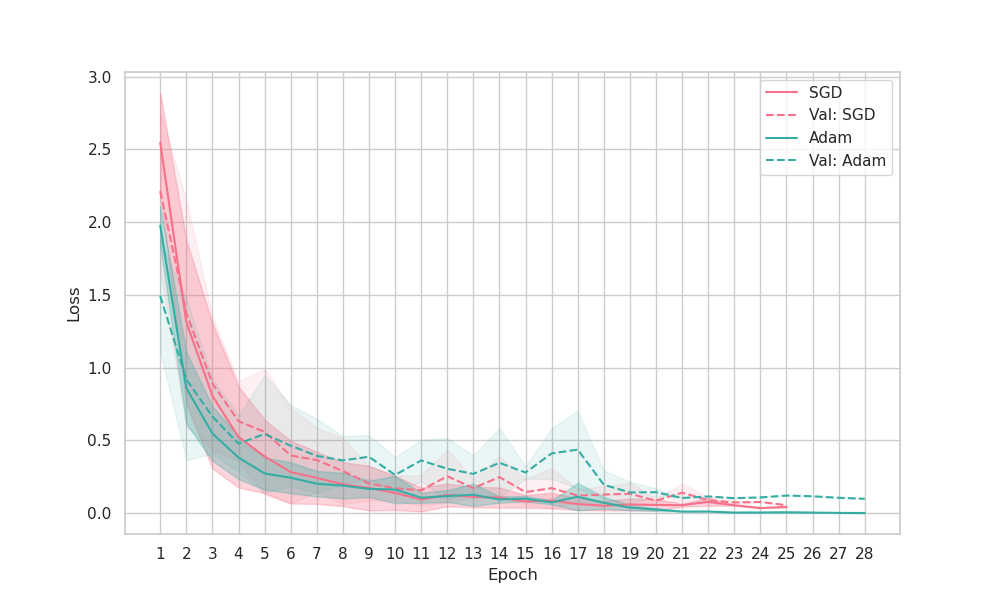
\includegraphics[width=0.8\textwidth]{img/loss-optimizer-marca.png}
	\caption{Función de pérdida promedio en entrenamiento y validación de los
		distintos modelos entrenados en función del optimizador empleado: SGD y Adam.
		Se muestra de forma sombreada la desviación típica de la función de pérdida.}
	\label{fig:loss-optim-m}
\end{figure}

Por otro lado, la \autoref{fig:loss-batch-m} muestra como existe una mayor
variabilidad en el proceso de entrenamiento entre los modelos con un mismo
tamaño de lote. Entre ellos, el que parece presentar una mayor estabilidad para
las distintas arquitecturas es con un tamaño de lote 64, pues muestra una menor desviación
típica y valores bajos en la función de pérdida.

\begin{figure}[H]
	\centering
	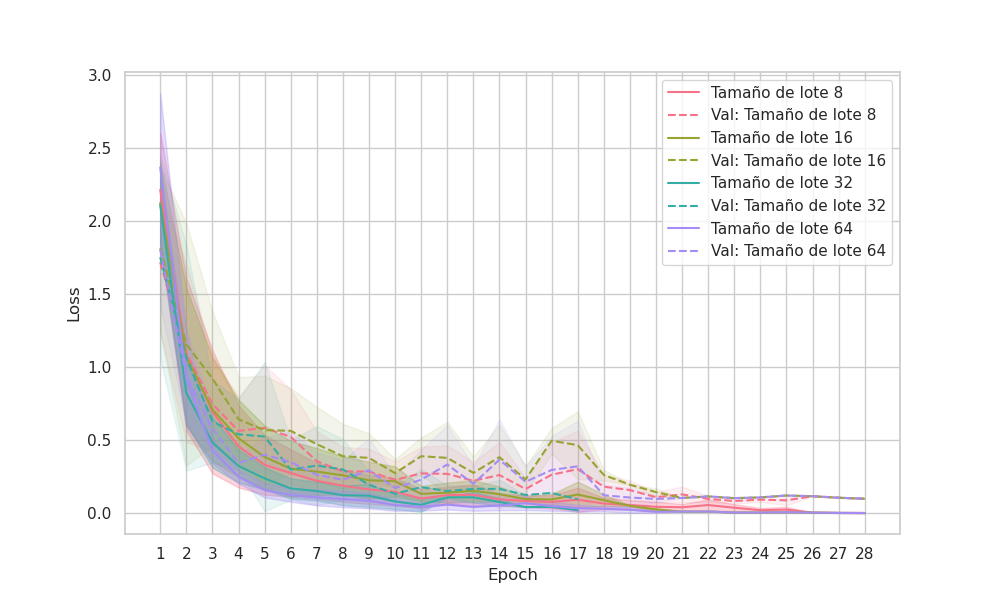
\includegraphics[width=0.8\textwidth]{img/loss-batch-marca.png}
	\caption{Función de pérdida promedio en entrenamiento y validación de los
		distintos modelos entrenados en función delos tamaños de lote empleados: 8, 16
		,32 y 64. Se muestra de forma sombreada la desviación típica de la función de pérdida.}
	\label{fig:loss-batch-m}
\end{figure}

Finalmente, las Figuras \ref{fig:loss-optim-mm} y \ref{fig:loss-batch-mm},
muestran un comportamiento similar a las recién vistas, indicando un correcto desarrollo
de la fase de entrenamiento. A diferencia de las anteriores, si bien SGD ha vuelto
a mostrar una mejor evolución de la curva de pérdida, es esta vez el tamaño de
lote 32 el que ha mostrado unas tasas de pérdida promedio más baja. Otra observación
interesante es la disminución en la pendiente de la curva, reflejando una mayor
dificultad en el aprendizaje en la especificidad Marca-Modelo.

\begin{figure}[H]
	\centering
	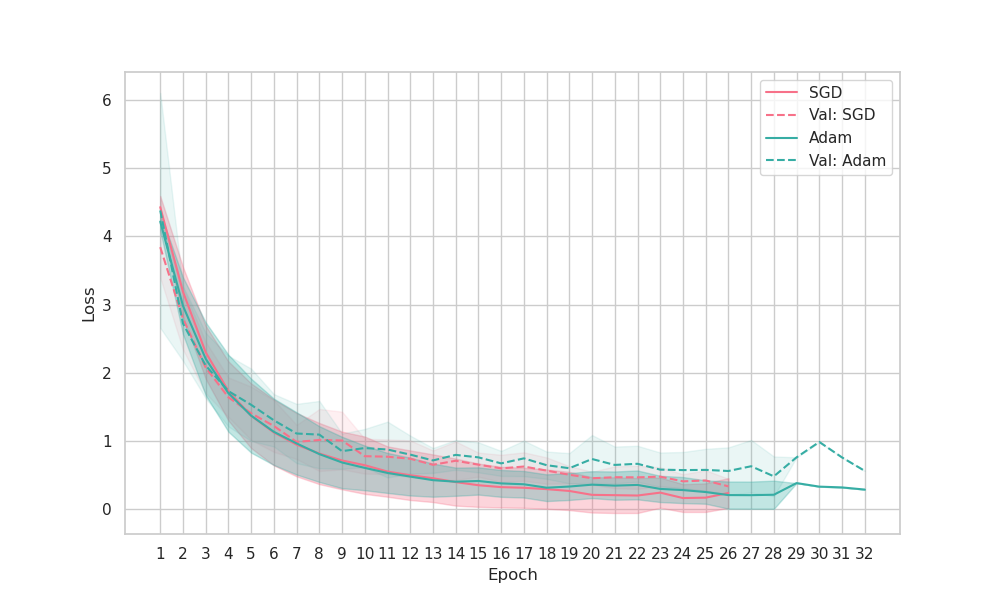
\includegraphics[width=0.8\textwidth]{img/loss-optimizer-marca-modelo.png}
	\caption{Función de pérdida promedio en entrenamiento y validación de los
		distintos modelos entrenados en función del optimizador empleado: SGD y Adam.
		Se muestra de forma sombreada la desviación típica de la función de pérdida.}
	\label{fig:loss-optim-mm}
\end{figure}

\begin{figure}[H]
	\centering
	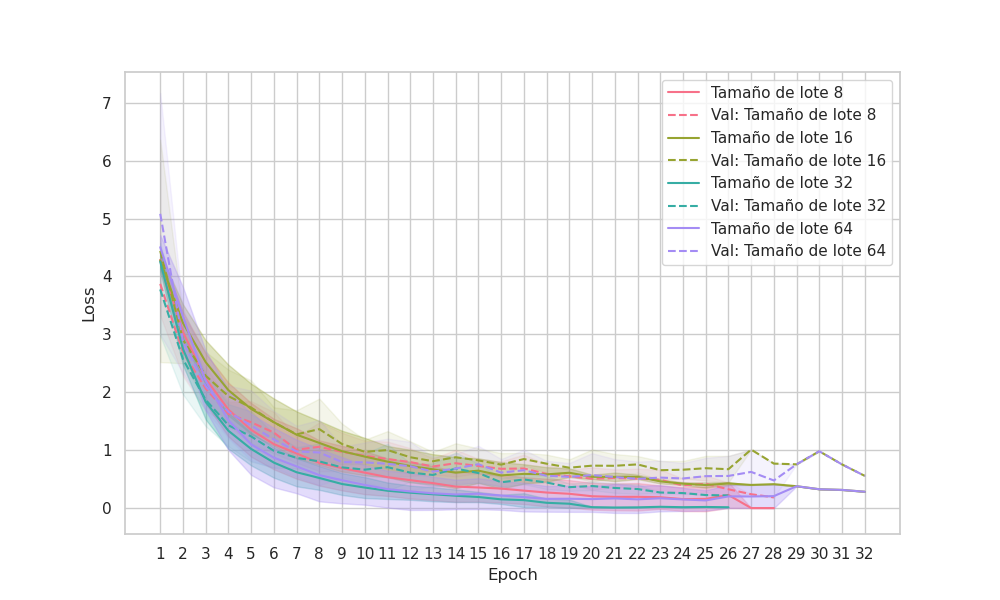
\includegraphics[width=0.8\textwidth]{img/loss-batch-marca-modelo.png}
	\caption{Función de pérdida promedio en entrenamiento y validación de los
		distintos modelos entrenados en función de los tamaños de lote empleados: 8,
		16 ,32 y 64. Se muestra de forma sombreada la desviación típica de la función de
		pérdida.}
	\label{fig:loss-batch-mm}
\end{figure}

Las Tablas \ref{tab:sgd_metrics-marca} y \ref{tab:adam_metrics-marca} muestran
las métricas obtenidas durante el proceso de entrenamiento tanto para SGD como
Adam respectivamente para la especificidad de Marca. Todas ellas han alcanzado el
criterio de parada en menos de 2 horas y de 50 épocas. En general, podemos observar
que ambos optimizadores logran una puntuación superior al $95\%$ en la gran mayoría
de las métricas. Es interesante observar cómo pese al desbalance de los datos, el
F1-Score sigue mostrando resultados excelentes. Entre todos los modelos vemos
que los mejores resultados los ha obtenido EfficientNet-B0 con el optimizador
SGD y un tamaño de lote 8 y 64. Sin embargo, finalmente se ha optado por escoger
el mismo modelo con un tamaño de lote 64, pues su resultados son muy similares y
su F1-Score es ligeramente mayor.

\begin{table}[H]
	\begin{adjustbox}
		{width=1\textwidth}
		\begin{tabular}{|c|c|c|c|c|c|}
			\hline
			\textbf{Modelo}             & \textbf{Tamaño de Lote} & \textbf{Exactitud} & \textbf{Precisión} & \textbf{Sensibilidad} & \textbf{F1-Score} \\
			\hline
			& 8                       & 0.9536             & 0.9416             & 0.9474                & 0.9443            \\
			\cline{2-6} ResNet-18       & 16                      & 0.9102             & 0.8834             & 0.8953                & 0.8891            \\
			\cline{2-6}                 & 32                      & 0.9721             & 0.9785             & 0.9753                & 0.9769            \\
			\cline{2-6}                 & 64                      & 0.9814             & 0.9758             & 0.9775                & 0.9767            \\
			\hline
			& 8                       & 0.9814             & 0.9850             & 0.9828                & 0.9838            \\
			\cline{2-6} DenseNet-121    & 16                      & 0.9752             & 0.9755             & 0.9783                & 0.9768            \\
			\cline{2-6}                 & 32                      & 0.9845             & 0.9931             & 0.9863                & 0.9897            \\
			\cline{2-6}                 & 64                      & 0.9814             & 0.9738             & 0.9753                & 0.9746            \\
			\hline
			& 8                       & \textbf{0.9907}    & 0.9907             & \textbf{0.9917}       & 0.9911            \\
			\cline{2-6} EfficientNet-B0 & 16                      & 0.9474             & 0.9512             & 0.9515                & 0.9512            \\
			\cline{2-6}                 & 32                      & 0.9690             & 0.9798             & 0.9689                & 0.9743            \\
			\cline{2-6}                 & 64                      & 0.9859             & \textbf{0.9925}    & 0.9907                & \textbf{0.9916}   \\
			\hline
		\end{tabular}
	\end{adjustbox}
	\caption{Métricas de validación para los modelos optimizados con SGD en la
		especificidad Marca.}
	\label{tab:sgd_metrics-marca}
\end{table}

\begin{table}[H]
	\begin{adjustbox}
		{width=1\textwidth}
		\begin{tabular}{|c|c|c|c|c|c|}
			\hline
			\textbf{Modelo}             & \textbf{Tamaño de Lote} & \textbf{Exactitud} & \textbf{Precisión} & \textbf{Sensibilidad} & \textbf{F1-Score} \\
			\hline
			& 8                       & 0.9536             & 0.9496             & 0.9508                & 0.9501            \\
			\cline{2-6} ResNet-18       & 16                      & 0.9536             & 0.9486             & 0.9467                & 0.9475            \\
			\cline{2-6}                 & 32                      & 0.9381             & 0.9319             & 0.9235                & 0.9275            \\
			\cline{2-6}                 & 64                      & 0.9721             & 0.9713             & 0.9633                & 0.9672            \\
			\hline
			& 8                       & 0.9350             & 0.9428             & 0.9363                & 0.9393            \\
			\cline{2-6} DenseNet-121    & 16                      & 0.9536             & 0.9465             & 0.9463                & 0.9462            \\
			\cline{2-6}                 & 32                      & 0.9659             & 0.9750             & 0.9694                & 0.9721            \\
			\cline{2-6}                 & 64                      & \textbf{0.9876}    & \textbf{0.9916}    & \textbf{0.9869}       & \textbf{0.9892}   \\
			\hline
			& 8                       & 0.9598             & 0.9588             & 0.9576                & 0.9580            \\
			\cline{2-6} EfficientNet-B0 & 16                      & 0.9752             & 0.9768             & 0.9757                & 0.9762            \\
			\cline{2-6}                 & 32                      & 0.9783             & 0.9720             & 0.9698                & 0.9709            \\
			\cline{2-6}                 & 64                      & 0.9567             & 0.9330             & 0.9332                & 0.9331            \\
			\hline
		\end{tabular}
	\end{adjustbox}
	\caption{Métricas de validación para los modelos optimizados con Adam en la
		especificidad Marca.}
	\label{tab:adam_metrics-marca}
\end{table}

Por otro lado, los modelos entrenados sobre el conjunto de datos Marca-Modelo han
mostrado mayores dificultades durante el proceso de aprendizaje, tal y como
muestran los resultados de las Tablas \ref{tab:sgd_metrics_mm} y
\ref{tab:adam_metrics_mm}. Pese a ello, la configuración que ha mostrado mejores
resultados en las métricas evaluadas ha sido DenseNet-121 con SGD y un tamaño de
lote 32. Esta configuración ha mostrado ser la mejor tanto en exactitud como en
F1-Score, además de tener resultados competentes en el resto de métricas. Por
ello, emplearemos dicho modelo en las siguientes etapas.

\begin{table}[H]
	\centering
	\begin{adjustbox}
		{width=\textwidth}
		\begin{tabular}{|c|c|c|c|c|c|}
			\hline
			\textbf{Modelo}             & \textbf{Tamaño de Lote} & \textbf{Exactitud} & \textbf{Precisión} & \textbf{Sensibilidad} & \textbf{F1-Score} \\
			\hline
			& 8                       & 0.8000             & 0.7934             & 0.7968                & 0.7949            \\
			\cline{2-6} ResNet-18       & 16                      & 0.8037             & 0.7866             & 0.7969                & 0.7916            \\
			\cline{2-6}                 & 32                      & 0.9000             & 0.8743             & 0.8912                & 0.8826            \\
			\cline{2-6}                 & 64                      & 0.8741             & 0.8510             & 0.8540                & 0.8524            \\
			\hline
			& 8                       & 0.8667             & 0.8569             & 0.8624                & 0.8595            \\
			\cline{2-6} DenseNet-121    & 16                      & 0.8741             & 0.8739             & 0.8732                & 0.8734            \\
			\cline{2-6}                 & 32                      & \textbf{0.9407}    & \textbf{0.9176}    & \textbf{0.9314}       & \textbf{0.9243}   \\
			\cline{2-6}                 & 64                      & 0.9111             & 0.8985             & 0.9009                & 0.8997            \\
			\hline
			& 8                       & 0.9111             & 0.9122             & 0.9116                & 0.9118            \\
			\cline{2-6} EfficientNet-B0 & 16                      & 0.8000             & 0.8020             & 0.8066                & 0.8040            \\
			\cline{2-6}                 & 32                      & 0.9148             & 0.9213             & 0.9181                & 0.9197            \\
			\cline{2-6}                 & 64                      & 0.9000             & 0.8941             & 0.8920                & 0.8929            \\
			\hline
		\end{tabular}
	\end{adjustbox}
	\caption{Métricas de validación para los modelos optimizados con SGD en la
		especificidad Marca-Modelo.}
	\label{tab:sgd_metrics_mm}
\end{table}

\begin{table}[H]
	\centering
	\begin{adjustbox}
		{width=\textwidth}
		\begin{tabular}{|c|c|c|c|c|c|}
			\hline
			\textbf{Modelo}             & \textbf{Tamaño de Lote} & \textbf{Exactitud} & \textbf{Precisión} & \textbf{Sensibilidad} & \textbf{F1-Score} \\
			\hline
			& 8                       & 0.8556             & 0.8526             & 0.8536                & 0.8529            \\
			\cline{2-6} ResNet-18       & 16                      & 0.8556             & 0.8471             & 0.8543                & 0.8506            \\
			\cline{2-6}                 & 32                      & 0.7741             & 0.7367             & 0.7561                & 0.7461            \\
			\cline{2-6}                 & 64                      & 0.8556             & 0.8493             & 0.8438                & 0.8464            \\
			\hline
			& 8                       & 0.8741             & 0.8672             & 0.8725                & 0.8696            \\
			\cline{2-6} DenseNet-121    & 16                      & 0.8667             & 0.8685             & 0.8687                & 0.8685            \\
			\cline{2-6}                 & 32                      & 0.9037             & 0.8943             & 0.9018                & 0.8979            \\
			\cline{2-6}                 & 64                      & \textbf{0.9201}    & \textbf{0.9263}    & 0.9103                & \textbf{0.9182}   \\
			\hline
			& 8                       & 0.8481             & 0.8384             & 0.8460                & 0.8420            \\
			\cline{2-6} EfficientNet-B0 & 16                      & 0.8926             & 0.8946             & 0.8924                & 0.8935            \\
			\cline{2-6}                 & 32                      & 0.9148             & 0.9044             & \textbf{0.9143}       & 0.9093            \\
			\cline{2-6}                 & 64                      & 0.8111             & 0.7869             & 0.7906                & 0.7887            \\
			\hline
		\end{tabular}
	\end{adjustbox}
	\caption{Métricas de validación para los modelos optimizados con Adam en la
		especificidad Marca-Modelo.}
	\label{tab:adam_metrics_mm}
\end{table}

\subsection{Selección de transformaciones de datos}

Tras la anterior etapa se ha procedido a realizar un aumento de datos sobre los
dos conjuntos seleccionados: EfficientNet-B0 con SGD y un tamaño de lote 64 para
la especificidad Marca, y DenseNet-121 con SGD y tamaño de lote 32 para la
especificidad Marca-Modelo. Las Tablas \ref{tab:transformation_metrics-m} y \ref{tab:transformation_metrics-mm}
muestran los resultados obtenidos para cada una de las transformaciones descritas
en la \autoref{sec:data-aug}.

Si bien el modelo entrenado para el conjunto de datos Marca con las transformaciones
no ha mejorado significativamente, vemos que las transformaciones sobre el
modelo entrenado para Marca-Modelo han logrado unas mejoras notablemente. El objetivo
del aumento de datos en las CNNs es mejorar la capacidad de generalización de los
modelos. Sin embargo, el primer modelo ya gozaba de muy buenas métricas por lo que
un empeoramiento general al realizar aumento de datos podría significar un sobreajuste
del modelo. Por tanto, entrenaremos el modelo de nuevo con las transformaciones que
mejor hayan funcionado para estudiar cómo afectan a la topología.

\begin{table}[H]
	\centering
	\begin{adjustbox}
		{width=0.8\textwidth}
		\begin{tabular}{|c|c|c|c|c|c|}
			\hline
			\textbf{Transformación} & \textbf{Exactitud} & \textbf{Precisión} & \textbf{Sensibilidad} & \textbf{F1-Score} \\
			\hline
			Fluctuación             & \textbf{0.9814}    & \textbf{0.9869}    & \textbf{0.9844}       & \textbf{0.9856}   \\
			\hline
			Desenfoque              & 0.9567             & 0.9360             & 0.9388                & 0.9373            \\
			\hline
			Simetría                & 0.9721             & 0.9634             & 0.9585                & 0.9609            \\
			\hline
			Recorte                 & 0.9783             & 0.9765             & 0.9709                & 0.9737            \\
			\hline
			Rotación                & 0.9783             & 0.9706             & 0.9657                & 0.9682            \\
			\hline
		\end{tabular}
	\end{adjustbox}
	\caption{Métricas de validación para EfficientNet-B0 con transformaciones de
		datos en la especificidad Marca.}
	\label{tab:transformation_metrics-m}
\end{table}

\begin{table}[H]
	\centering
	\begin{adjustbox}
		{width=0.8\textwidth}
		\begin{tabular}{|c|c|c|c|c|c|}
			\hline
			\textbf{Transformación} & \textbf{Exactitud} & \textbf{Precisión} & \textbf{Sensibilidad} & \textbf{F1-Score} \\
			\hline
			Fluctuación             & 0.9783             & 0.9728             & 0.9745                & 0.9736            \\
			\hline
			Desenfoque              & 0.9783             & 0.9790             & 0.9750                & 0.9769            \\
			\hline
			Simetría                & 0.9814             & 0.9804             & 0.9775                & 0.9789            \\
			\hline
			Recorte                 & 0.9845             & 0.9863             & 0.9817                & 0.9840            \\
			\hline
			Rotación                & \textbf{0.9876}    & \textbf{0.9914}    & \textbf{0.9874}       & \textbf{0.9894}   \\
			\hline
		\end{tabular}
	\end{adjustbox}
	\caption{Métricas de validación para DenseNet-121 con transformaciones de
		datos en la especificidad Marca-Modelo.}
	\label{tab:transformation_metrics-mm}
\end{table}

Finalmente, la \autoref{tab:model_comparison_val} muestra los resultados de los
modelos reentrenados con las transformaciones escogidas: EfficientNet-B0 con fluctuaciones
en el color, recortes aleatorios y rotaciones aleatorias en Marca; y DenseNet-121
con todas las transformaciones propuestas en Marca-Modelo.

\begin{table}[H]
	\centering
	\begin{adjustbox}
		{width=0.85\textwidth}
		\begin{tabular}{|c|c|c|c|c|}
			\hline
			\textbf{Modelo}                   & \textbf{Exactitud} & \textbf{Precisión} & \textbf{Sensibilidad} & \textbf{F1-Score} \\
			\hline
			EfficientNet-B0 Trans (Marca)     & 0.9505             & 0.9627             & 0.9501                & 0.9562            \\
			\hline
			\hline
			DenseNet-121 Trans (Marca-Modelo) & 0.7962             & 0.7660             & 0.7769                & 0.7712            \\
			\hline
		\end{tabular}
	\end{adjustbox}
	\caption{Rendimiento final de los modelos con aumento de datos en el conjunto
		de validación para EfficientNet-B0 en la especificidad Marca y para DenseNet-121
		en la especificidad Marca-Modelo. }
	\label{tab:model_comparison_val}
\end{table}

Una vez obtenidos los modelos, podemos observar en la \autoref{tab:model_comparison_test_aug}
las métricas obtenidas en cada modelo en el conjunto de test, tanto el modelo
base como el de aumento de datos. Es especialmente interesante el comportamiento
de DenseNet-121 con aumento de datos. Pese a tener bajos resultados en el
conjunto de validación, ha mostrado una buena generalización en el conjunto de test,
incluso superando al modelo base.

\begin{table}[H]
	\centering
	\begin{adjustbox}
		{width=0.85\textwidth}
		\begin{tabular}{|c|c|c|c|c|}
			\hline
			\textbf{Modelo}                   & \textbf{Exactitud} & \textbf{Precisión} & \textbf{Sensibilidad} & \textbf{F1-Score} \\
			\hline
			EfficientNet-B0 Base (Marca)      & \textbf{0.9505}    & \textbf{0.9462}    & \textbf{0.9386}       & \textbf{0.9423}   \\
			\hline
			EfficientNet-B0 Trans (Marca)     & 0.9474             & 0.9319             & 0.9271                & 0.9294            \\
			\hline
			\hline
			DenseNet-121 Base (Marca-Modelo)  & 0.9185             & 0.9077             & 0.9126                & 0.9101            \\
			\hline
			DenseNet-121 Trans (Marca-Modelo) & \textbf{0.9474}    & \textbf{0.9319}    & \textbf{0.9271}       & \textbf{0.9294}   \\
			\hline
		\end{tabular}
	\end{adjustbox}
	\caption{Rendimiento final de los modelos con y sin aumento de datos en el
		conjunto de test para EfficientNet-B0 en la especificidad Marca y para
		DenseNet-121 en la especificidad Marca-Modelo.}
	\label{tab:model_comparison_test_aug}
\end{table}

\section{Análisis de la homología persistente}
\label{sec:homology-analysis}

Una vez habiendo entrenado todos los modelos necesarios, procederemos analizando
los resultados obtenidos en función de la homología persistente. Para ello, se ha
calculado la persistencia total de una muestra de 128 instancias (debido al
coste en memoria) del conjunto de test tras cada activación no lineal presente en
la red evaluada. Las gráficas empleadas a lo largo de toda la sección registran
tanto la persistencia total como la normalizada de la muestra frente a su
posición relativa en su paso por la red expresada en porcentaje. Además, las
figuras muestran la curva de regresión cuadrática calculada a partir de la
persistencia con el fin de una visualización más clara de la tendencia de dichos
valores. Las áreas sombreadas indican el intervalo de confianza del 95\%.

Las Secciones \ref{subsec:arch}, \ref{subsec:optim} y \ref{subsec:batch} realizan
un estudio comparativo en función de la arquitectura, optimizador y tamaño de
lote descritos en el \autoref{chapter:methodology}. Posteriormente, en las
Secciones \ref{subsec:aug}, \ref{subsec:grano} y \ref{subsec:set}, el análisis
se realiza a parir del mejor modelo para cada especificidad con el fin de
analizar cómo afectan el aumento de datos, la granularidad del conjunto y la partición
de datos escogida a la topología de estos.

\subsection{Comparación según la arquitectura}
\label{subsec:arch}

\paragraph{Especificidad Marca}

Comencemos analizando la \autoref{fig:m-homology-arch-1}. La gráfica muestra una
tendencia clara entre los modelos estudiados con los diferentes hiperparámetros:
una disminución pronunciada de la persistencia total con un leve repunte en la
etapa final de ejecución. Esto implica que las transformaciones que realiza el modelo
sobre el conjunto de instancias (como los cambios en dimensionalidad y las
funciones aplicadas sobre ellos) tienden tanto a disminuir la persistencia de las
clases de homología como a reducir el número de ellos que se generan, claramente
simplificando los datos. Un comportamiento interesante es el obtenido al final de
las ejecuciones, donde los modelos complican la homología persistente de los
datos de cara a la tarea de clasificación final, aumentando la persistencia de componentes
conexas y otras características topológicas más complejas, con el fin de
facilitar la separación de clases final.

Asimismo, la \autoref{fig:m-homology-arch-2} muestra una conclusiones similares con
otra tendencia: la persistencia homológica de los datos crece durante las
primeras fases de la inferencia, mientras que desciende de cara al final de la ejecución.
Es decir, las clases de homología persistente tienden a ser más homogéneas en el
punto medio de la ejecución, de forma que los datos están más dispersos y
desordenados. De no ser así, las componentes conexas y clases de homología
persistentes en dimensión 1 morirían en fases tempranas de la filtración, lo que
daría una persistencia total normalizada más baja.

\begin{figure}[H]
	\centering
	\begin{subfigure}
		{.5\textwidth}
		\centering
		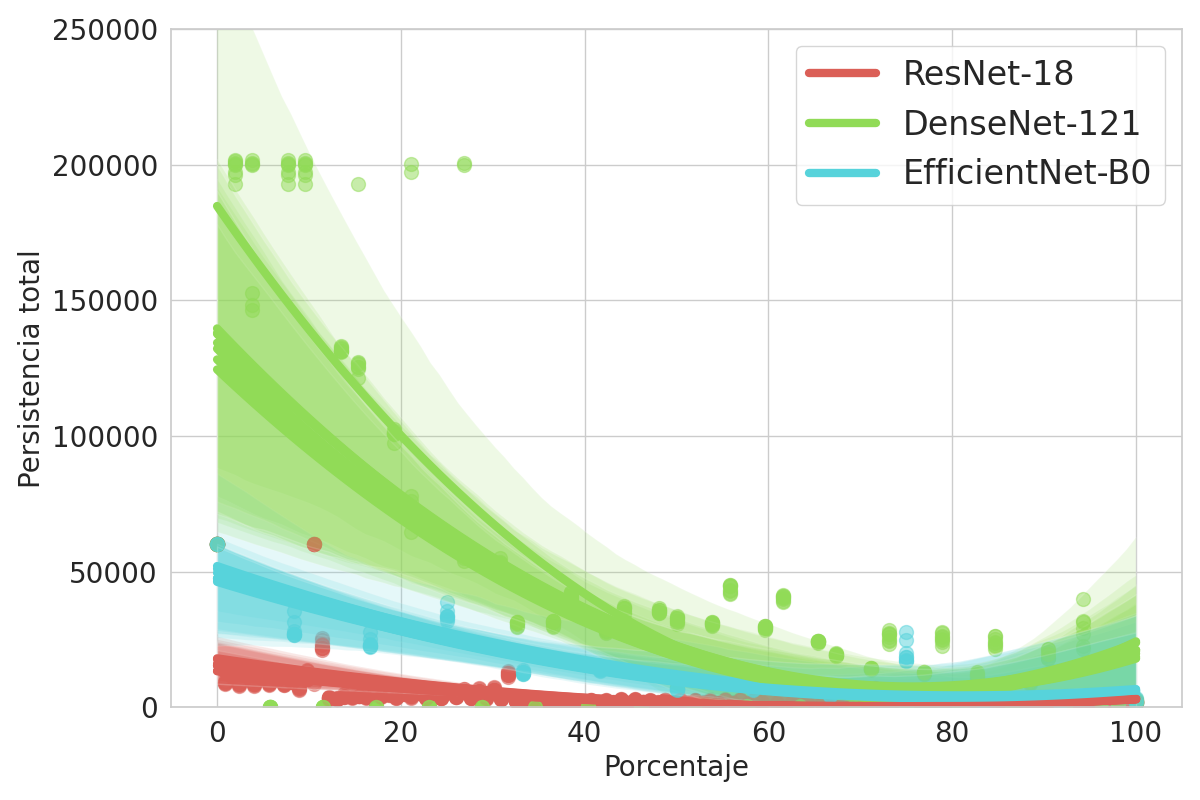
\includegraphics[width=\linewidth]{img/m_arch.png}
		\caption{Persistencia total según el porcentaje de avance en las redes para
			los modelos ResNet-18, DenseNet-121 y EfficientNet-B0.}
		\label{fig:m-homology-arch-1}
	\end{subfigure}%
	\begin{subfigure}
		{.5\textwidth}
		\centering
		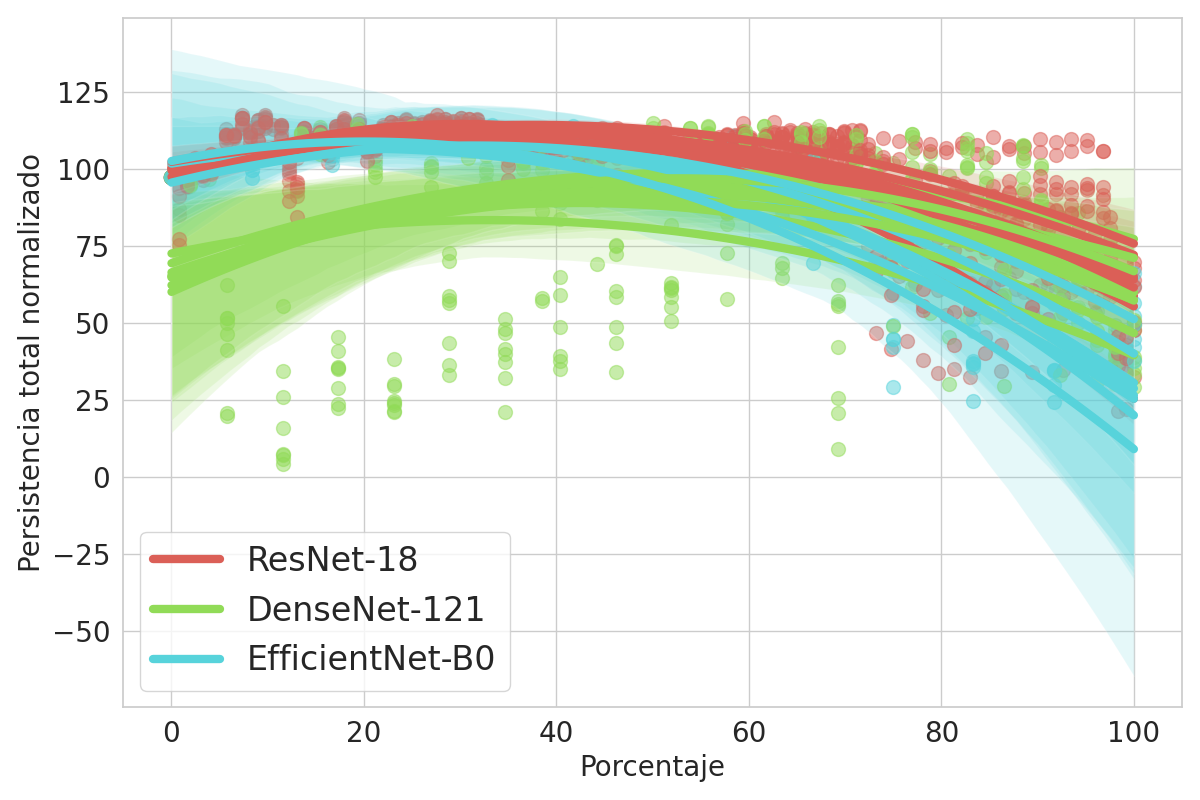
\includegraphics[width=\linewidth]{img/m_arch_norm.png}
		\caption{Persistencia total normalizada según el porcentaje de avance en las
			redes para los modelos ResNet-18, DenseNet-121 y EfficientNet-B0.}
		\label{fig:m-homology-arch-2}
	\end{subfigure}
	\caption{Comparación de la persistencia total (a) y la persistencia total
		normalizada (b) de diferentes arquitecturas de redes neuronales en función del
		porcentaje de avance de los datos a través de la red para la especificidad
		Marca-Modelo.}
	\label{fig:m-homology-arch}
\end{figure}

\paragraph{Especificidad Marca-Modelo}

Los resultados de las gráficas de la \autoref{fig:mm-homology-arch} muestran una
tendencia similar. En este caso, las tendencias del modelo DenseNet-121 en la
\autoref{fig:mm-homology-arch-1} muestran una pendiente más pronunciada, indicando
transformaciones más agresivas en la homología persistente de los datos. Por
otro lado, la \autoref{fig:mm-homology-arch-2} muestra un comportamiento algo diferente
respecto a la obtenida en la especificidad Marca, obteniendo unos valores de
persistencia total normalizada notablemente superiores al final de las
ejecuciones. Dicha consecuencia puede deberse al aumento en la granularidad de la
clasificación, haciendo necesarias un mayor número de componentes conexas para
facilitar dicha tarea.

\begin{figure}[H]
	\centering
	\begin{subfigure}
		{.5\textwidth}
		\centering
		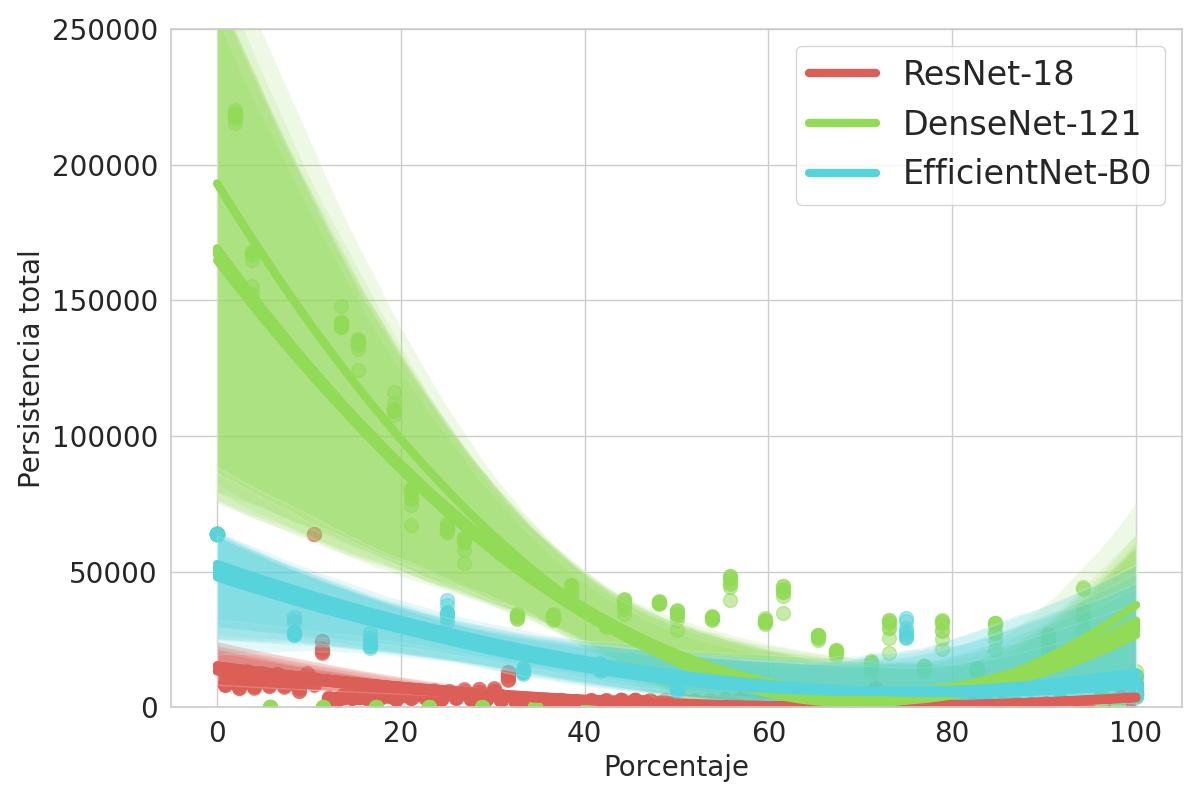
\includegraphics[width=\linewidth]{img/mm_arch.png}
		\caption{Persistencia total según el porcentaje de avance en las redes para
			los modelos ResNet-18, DenseNet-121 y EfficientNet-B0.}
		\label{fig:mm-homology-arch-1}
	\end{subfigure}%
	\begin{subfigure}
		{.5\textwidth}
		\centering
		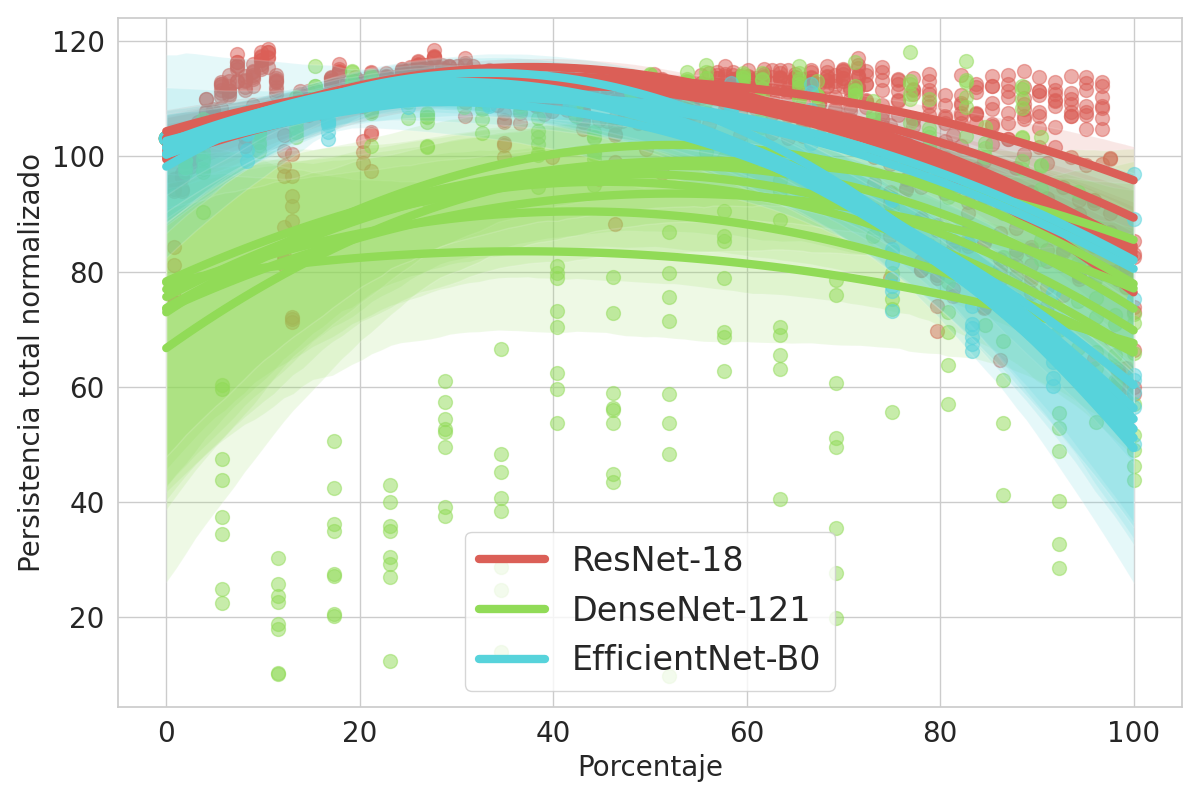
\includegraphics[width=\linewidth]{img/mm_arch_norm.png}
		\caption{Persistencia total normalizada según el porcentaje de avance en las
			redes para los modelos ResNet-18, DenseNet-121 y EfficientNet-B0.}
		\label{fig:mm-homology-arch-2}
	\end{subfigure}
	\caption{Comparación de la persistencia total (a) y la persistencia total
		normalizada (b) de diferentes arquitecturas de redes neuronales en función del
		porcentaje de avance de los datos a través de la red para la especificidad
		Marca-Modelo.}
	\label{fig:mm-homology-arch}
\end{figure}

Es claro que las Figuras \ref{fig:m-homology-arch} y \ref{fig:mm-homology-arch} indican
que la arquitectura escogida es un factor determinante en las transformaciones que
los datos sufren desde el punto de vista topológico. Todos los modelos
entrenados con la misma arquitectura muestran evoluciones muy similares incluso
para las distintas especificidades, donde si que se aprecia un desplazamiento vertical
de la homología persistente en función de la granularidad de las clases del conjunto.

\subsection{Comparación según el optimizador}
\label{subsec:optim}

\paragraph{Especificidad Marca}

A diferencia de la comparativa en función de la arquitectura, la \autoref{fig:m-homology-optim}
no muestra patrones tan claros en cómo afecta el optimizador a la persistencia homológica.
La \autoref{fig:m-homology-optim-1} muestra cómo los modelos que presentan una
menor persistencia total al inicio, como ResNet-18, tienden a presentar una
persistencia inicial todavía menor para el optimizador SGD. Sin embargo, esta
tendencia empieza a cambiar cuando vamos pasando a modelos de mayor complejidad
topológica como DenseNet-121, donde en general Adam parece mostrar una menor persistencia
inicial. Por otro lado, la \autoref{fig:m-homology-optim-2} no parece mostrar ningún
patrón que nos indique que la elección del optimizador sea relevante para la modificación
de la homología persistente de los datos.

\begin{figure}[H]
	\centering
	\begin{subfigure}
		{.5\textwidth}
		\centering
		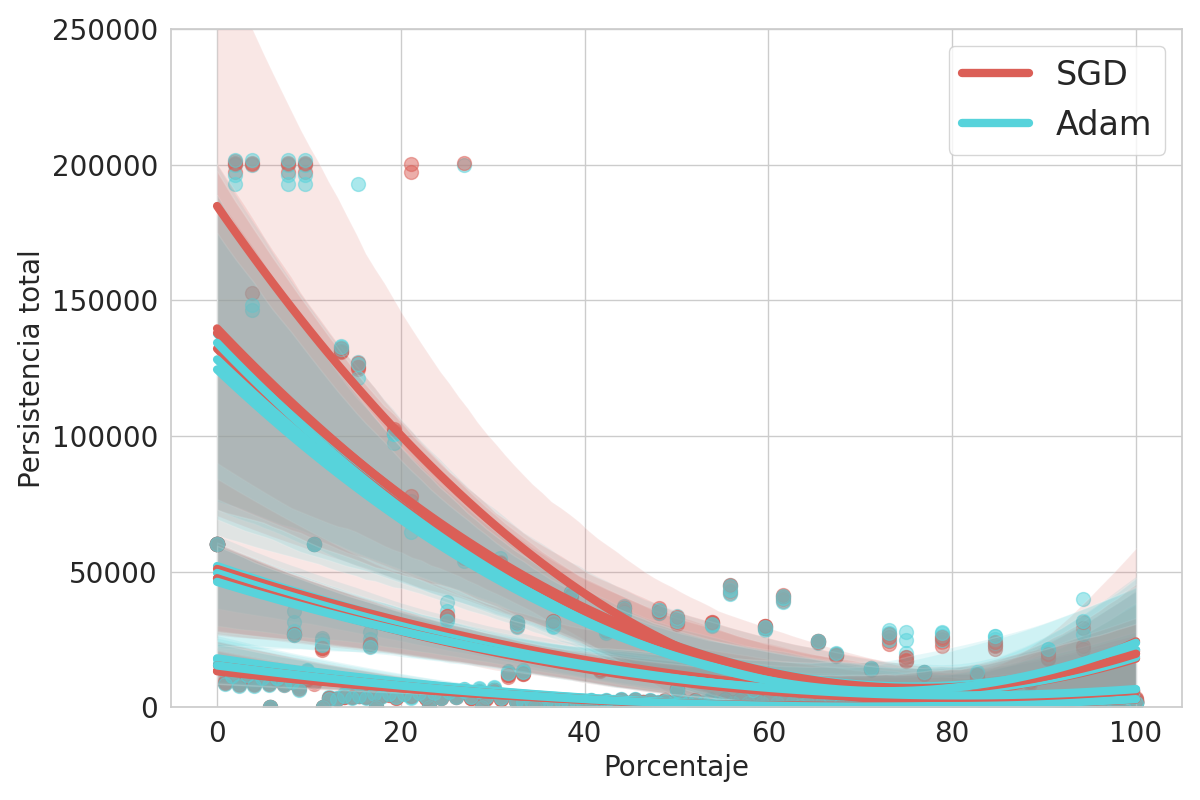
\includegraphics[width=\linewidth]{img/m_optim.png}
		\caption{Persistencia total según el porcentaje de avance en las redes para
			optimizadores SGD y Adam.}
		\label{fig:m-homology-optim-1}
	\end{subfigure}%
	\begin{subfigure}
		{.5\textwidth}
		\centering
		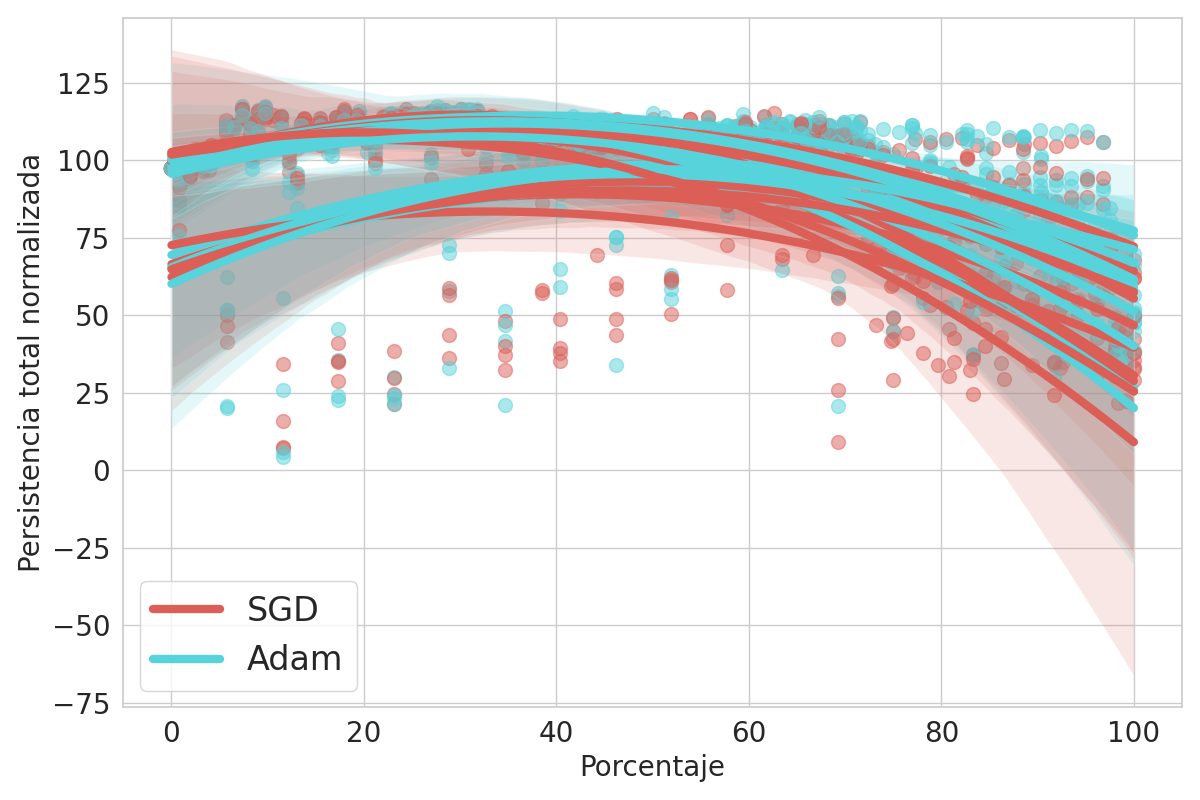
\includegraphics[width=\linewidth]{img/m_optim_norm.png}
		\caption{Persistencia total normalizada según el porcentaje de avance en las
			redes para SGD y Adam.}
		\label{fig:m-homology-optim-2}
	\end{subfigure}
	\caption{Comparación de la persistencia total (a) y la persistencia total
		normalizada (b) de diferentes optimizadores de redes neuronales en función del
		porcentaje de avance de los datos a través de la red para la especificidad
		Marca.}
	\label{fig:m-homology-optim}
\end{figure}

\paragraph{Especificidad Marca-Modelo}

De nuevo, los resultados obtenidos en la \autoref{fig:mm-homology-optim} son poco
esclarecedores acerca de la homología de los datos. No obstante, el aumento en el
número de clases parece haber homogeneizado las diferencias observadas en la persistencia
total, tal y como muestra la \autoref{fig:mm-homology-optim-1}. Además, las
tendencias en la \autoref{fig:mm-homology-optim-2} muestran una mayor
persistencia total normalizada al final de la inferencia para los modelos
entrenados con Adam.

\begin{figure}[H]
	\centering
	\begin{subfigure}
		{.5\textwidth}
		\centering
		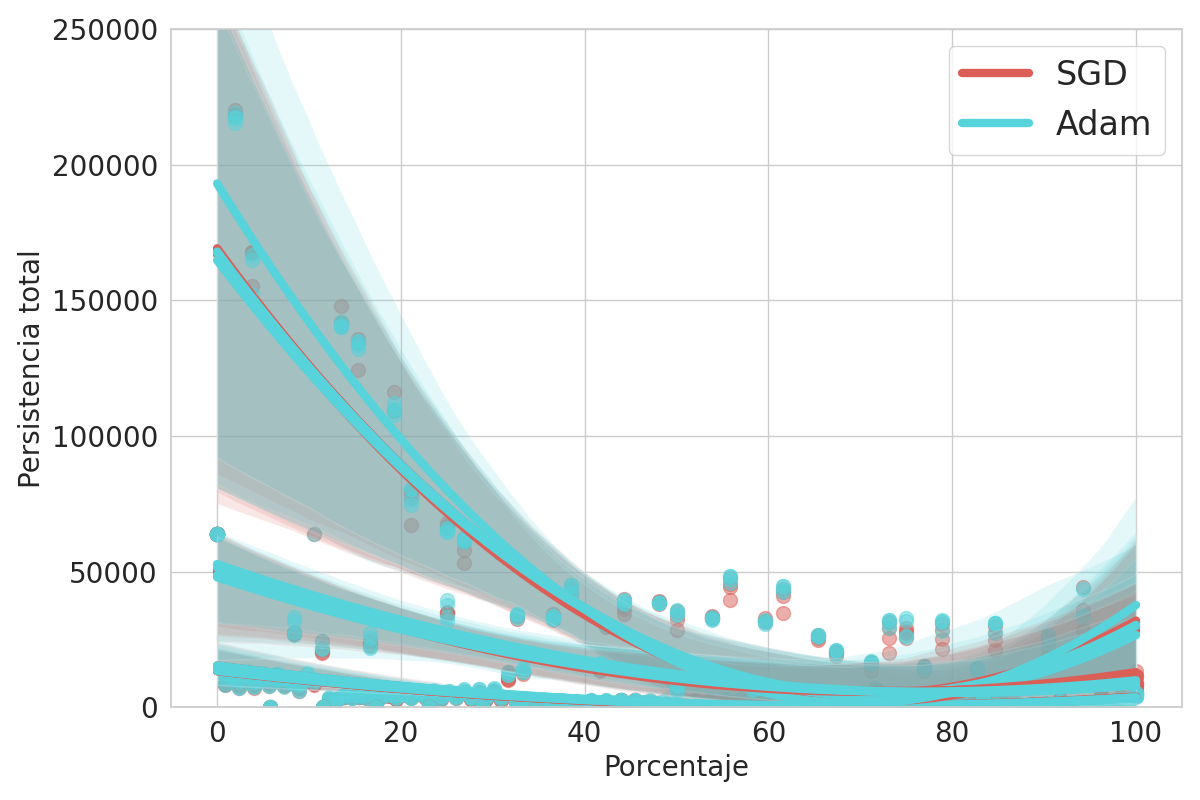
\includegraphics[width=\linewidth]{img/mm_optim.png}
		\caption{Persistencia total normalizada según el porcentaje de avance en la
			red para optimizadores SGD y Adam.}
		\label{fig:mm-homology-optim-1}
	\end{subfigure}%
	\begin{subfigure}
		{.5\textwidth}
		\centering
		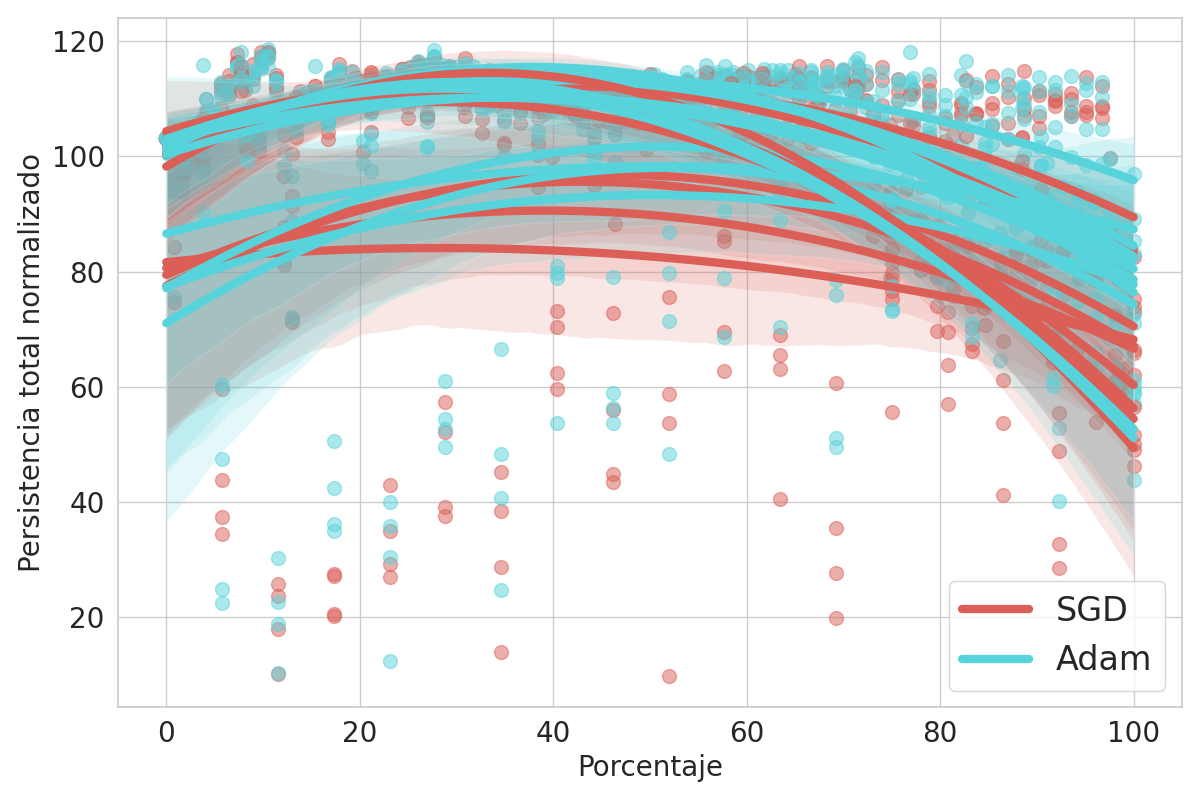
\includegraphics[width=\linewidth]{img/mm_optim_norm.png}
		\caption{Persistencia total normalizada según el porcentaje de avance en la
			red para optimizadores SGD y Adam.}
		\label{fig:mm-homology-optim-2}
	\end{subfigure}
	\caption{Comparación de la persistencia total (a) y la persistencia total
		normalizada (b) de diferentes optimizadores de redes neuronales en función del
		porcentaje de avance de los datos a través de la red para la especificidad
		Marca-Modelo.}
	\label{fig:mm-homology-optim}
\end{figure}

Los resultados recién vistos sobre las Figuras \ref{fig:m-homology-optim} y \ref{fig:mm-homology-optim}
parecen mostrar que el optimizador escogido (al menos, en el caso de los dos empleados)
no es un factor especialmente relevante a la hora de modificar la \enquote{forma}
de los datos. A pesar de ello, las tendencias observadas al inicio de la red en la
persistencia total y al final de ella en la persistencia total normalizada muestran
de manera débil ciertos patrones que podrían estudiarse en más profundidad.

\subsection{Comparación según el tamaño de lote}
\label{subsec:batch}

\paragraph{Especificidad Marca}

Las gráficas de la \autoref{fig:m-homology-batch} no muestran ninguna influencia
directa o significativa de la elección del tamaño de lote en el ámbito de la
topología de los datos durante la etapa de entrenamiento. Las curvas de regresión
se muestran muy entrelazadas y las nubes de puntos no muestran claras distinciones
o agrupaciones.

\begin{figure}[H]
	\centering
	\begin{subfigure}
		{.5\textwidth}
		\centering
		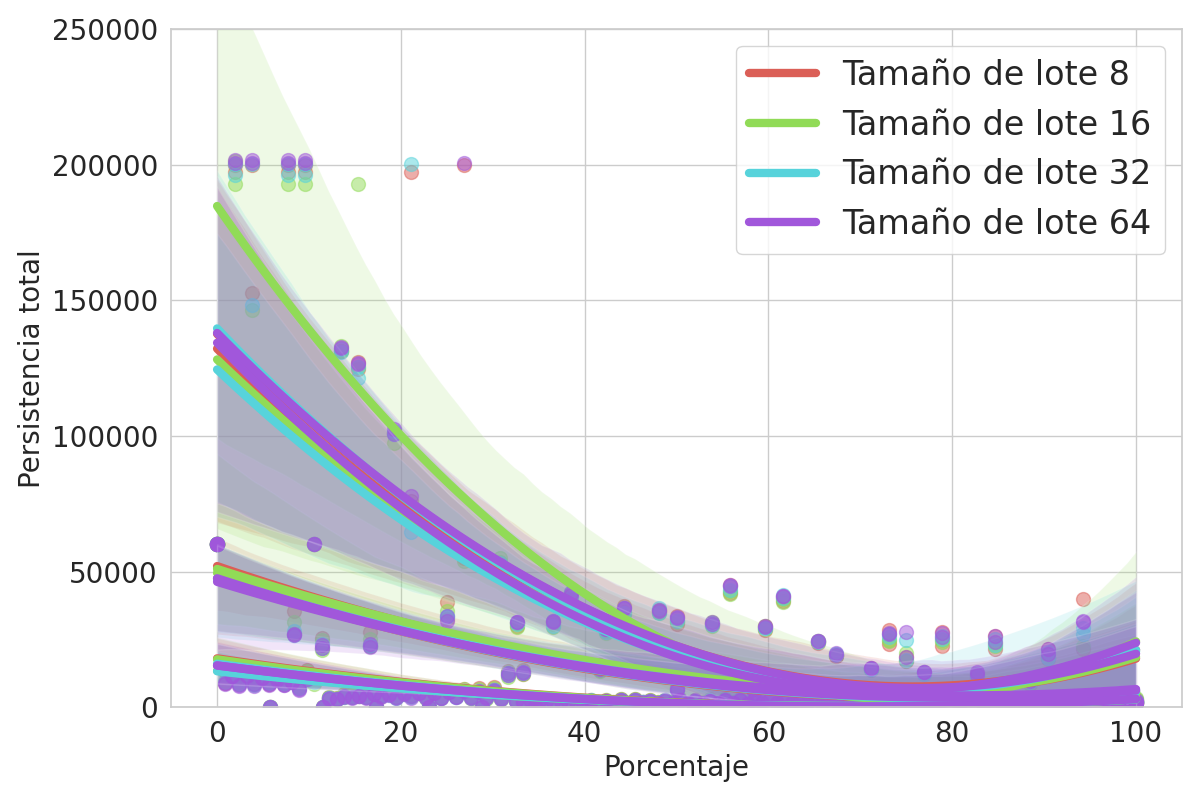
\includegraphics[width=\linewidth]{img/m_batch.png}
		\caption{Persistencia total según el porcentaje de avance en las redes
			entrenadas para diferentes tamaños de lote.}
		\label{fig:m-homology-batch-1}
	\end{subfigure}%
	\begin{subfigure}
		{.5\textwidth}
		\centering
		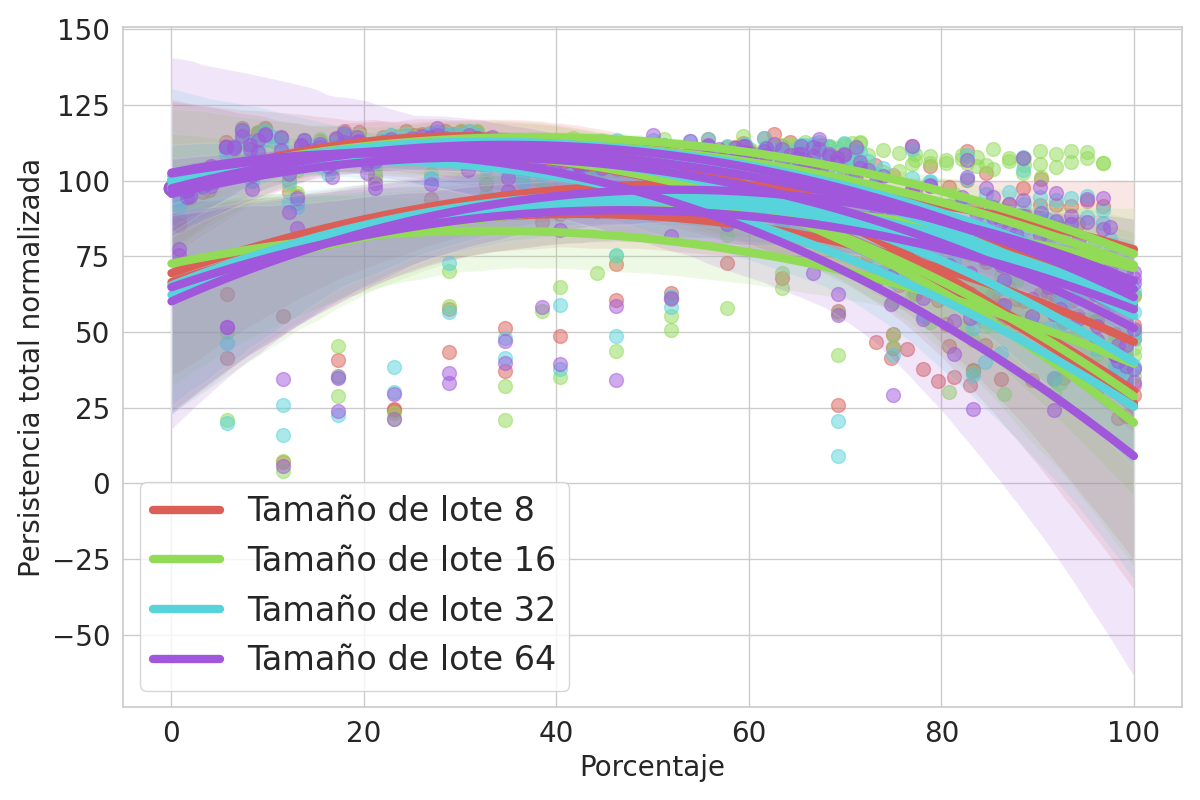
\includegraphics[width=\linewidth]{img/m_batch_norm.png}
		\caption{Persistencia total normalizada según el porcentaje de avance en las
			redes para diferentes tamaños de lote.}
		\label{fig:m-homology-batch-2}
	\end{subfigure}
	\caption{Comparación de la persistencia total (a) y la persistencia total
		normalizada (b) para diferentes tamaños de lote en función del porcentaje de
		avance de los datos a través de la red para la especificidad Marca.}
	\label{fig:m-homology-batch}
\end{figure}

\paragraph{Especificidad Marca-Modelo}

La misma observación se obtiene para los modelos entrenados en la especificidad
Marca-Modelo, donde las gráficas de la \autoref{fig:mm-homology-batch} muestran un
patrón bastante similar a las recién comentadas.

\begin{figure}[H]
	\centering
	\begin{subfigure}
		{.5\textwidth}
		\centering
		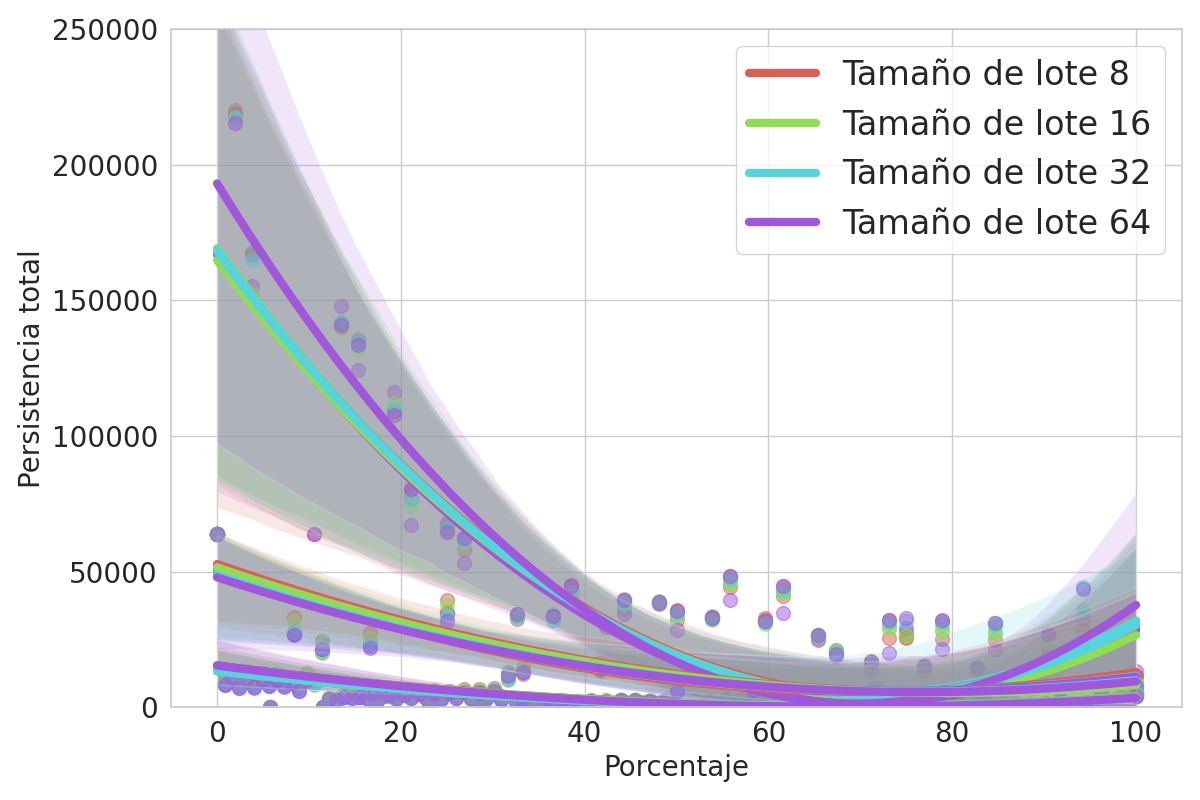
\includegraphics[width=\linewidth]{img/mm_batch.png}
		\caption{Persistencia total según el porcentaje de avance en las redes para
			diferentes tamaños de lote.}
		\label{fig:mm-homology-batch-1}
	\end{subfigure}%
	\begin{subfigure}
		{.5\textwidth}
		\centering
		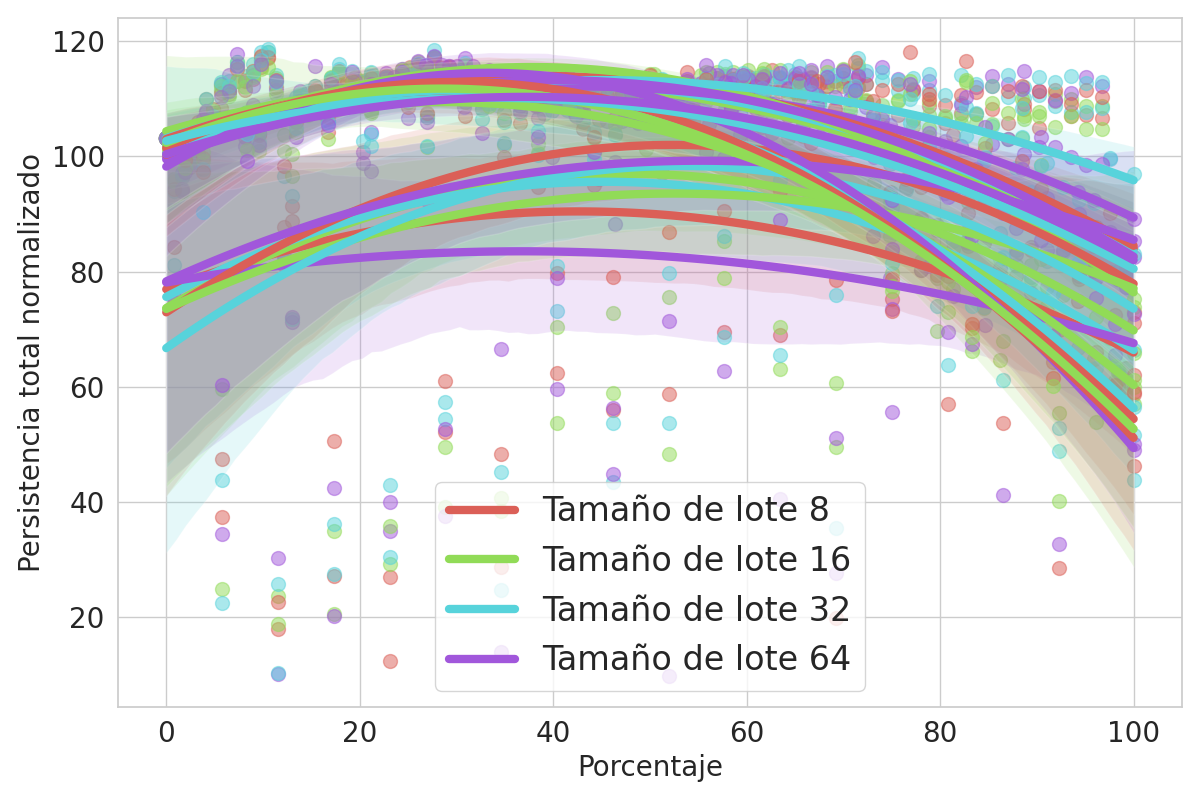
\includegraphics[width=\linewidth]{img/mm_batch_norm.png}
		\caption{Persistencia total normalizada según el porcentaje de avance en las
			redes para diferentes tamaños de lote.}
		\label{fig:mm-homology-batch-2}
	\end{subfigure}
	\caption{Comparación de la persistencia total (a) y la persistencia total
		normalizada (b) para diferentes tamaños de lote en función del porcentaje de
		avance de los datos a través de la red para la especificidad Marca-Modelo.}
	\label{fig:mm-homology-batch}
\end{figure}

Es curioso observar que esta elección de hiperparámetros no muestre alteraciones
en la homología persistente de los datos de test estudiados. Este hecho podría implicar
que los métodos de optimización empleados son poco sensibles al tamaño de lote escogido
a la hora de inferir la variedad subyacente de los datos.

\subsection{Comparación en presencia de aumento de datos}
\label{subsec:aug}

A continuación trabajaremos sobre los modelos escogidos en la
\autoref{subsec:hiperparam} para cada especificidad.

\paragraph{Especificidad Marca: EfficientNet-B0}

La \autoref{fig:m-homology} muestra los resultados de persistencia total y
persistencia total normalizada para el modelo base de EfficientNet-B0 y su
variante con aumento de datos. Podemos observar que el modelo que obtuvo mejores
métricas en el conjunto de test, el modelo base, presenta una persistencia total
superior tanto al inicio como al final respecto al modelo con aumento de datos,
mientras que es menor en el punto medio de la ejecución, tal y como se ve en la \autoref{fig:m-homology-1}.
Esto es, el modelo con mejores métricas muestra transformaciones más agresivas sobre
la variedad subyacente de los datos.

En cuanto a la \autoref{fig:m-homology-2}, vemos que el modelo con aumento de
datos presenta una persistencia total normalizada inicial más alta que el modelo
base y una final más baja. Además, vemos que el máximo de persistencia lo
alcanza antes que el modelo base, mostrando una traslación del proceso de aumento
de la complejidad en homología persistente a etapas más tempranas de la ejecución.

\begin{figure}[H]
	\centering
	\begin{subfigure}
		{.5\textwidth}
		\centering
		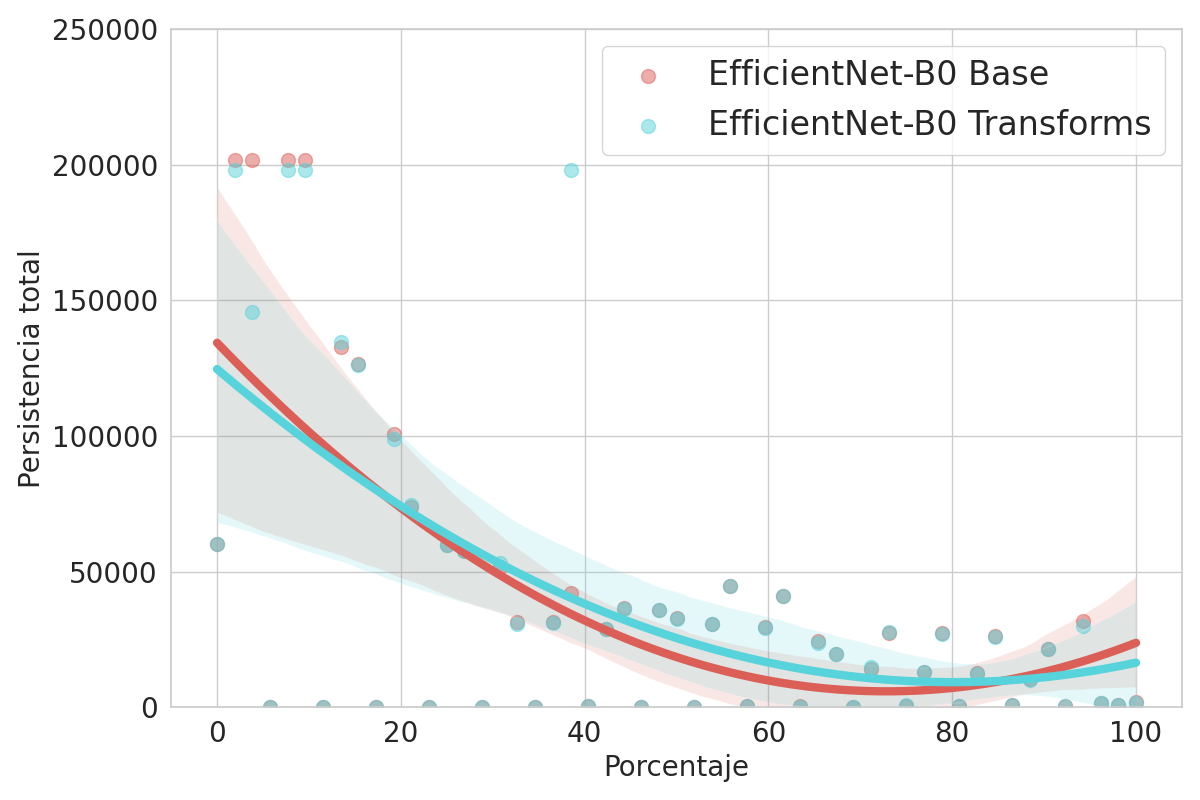
\includegraphics[width=\linewidth]{img/m.png}
		\caption{Persistencia total según el porcentaje de avance en la red para el
			modelo base entrenado EfficientNet-B0 y su versión con aumento de datos.}
		\label{fig:m-homology-1}
	\end{subfigure}%
	\begin{subfigure}
		{.5\textwidth}
		\centering
		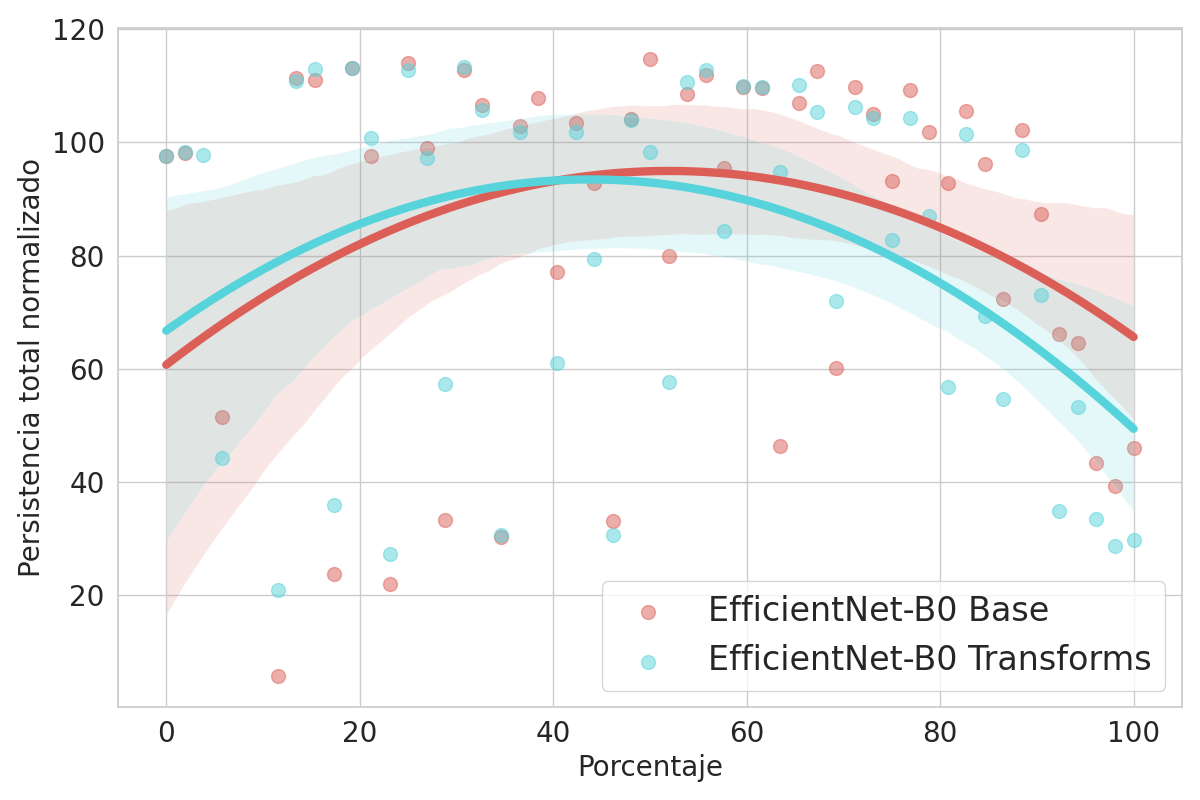
\includegraphics[width=\linewidth]{img/m_norm.png}
		\caption{Persistencia total normalizada según el porcentaje de avance en la
			red para el modelo base entrenado EfficientNet-B0 y su versión con aumento
			de datos.}
		\label{fig:m-homology-2}
	\end{subfigure}
	\caption{Comparación de la persistencia total (a) y la persistencia total
		normalizada (b) para EfficientNet-B0 Base y EfficientNet-B0 Transforms en
		función del porcentaje de avance de los datos a través de la red para la
		especificidad Marca.}
	\label{fig:m-homology}
\end{figure}

\paragraph{Especificidad Marca-Modelo: DenseNet-121}

Estas observaciones se ven reforzadas en la \autoref{fig:mm-homology}. En particular,
la \autoref{fig:mm-homology-1} muestra dichas observaciones de una manera más
agresiva. Vemos que el mejor modelo, DenseNet-121 con aumento de datos, muestra una
persistencia total mayor al inicio de la red y al final. Además, la \autoref{fig:mm-homology-2}
muestra como el aumento de datos traslada de nuevo el máximo a momentos más tempranos
de ejecución y una fuerte reducción de la complejidad total normalizada al final
de la red.

\begin{figure}[H]
	\centering
	\begin{subfigure}
		{.5\textwidth}
		\centering
		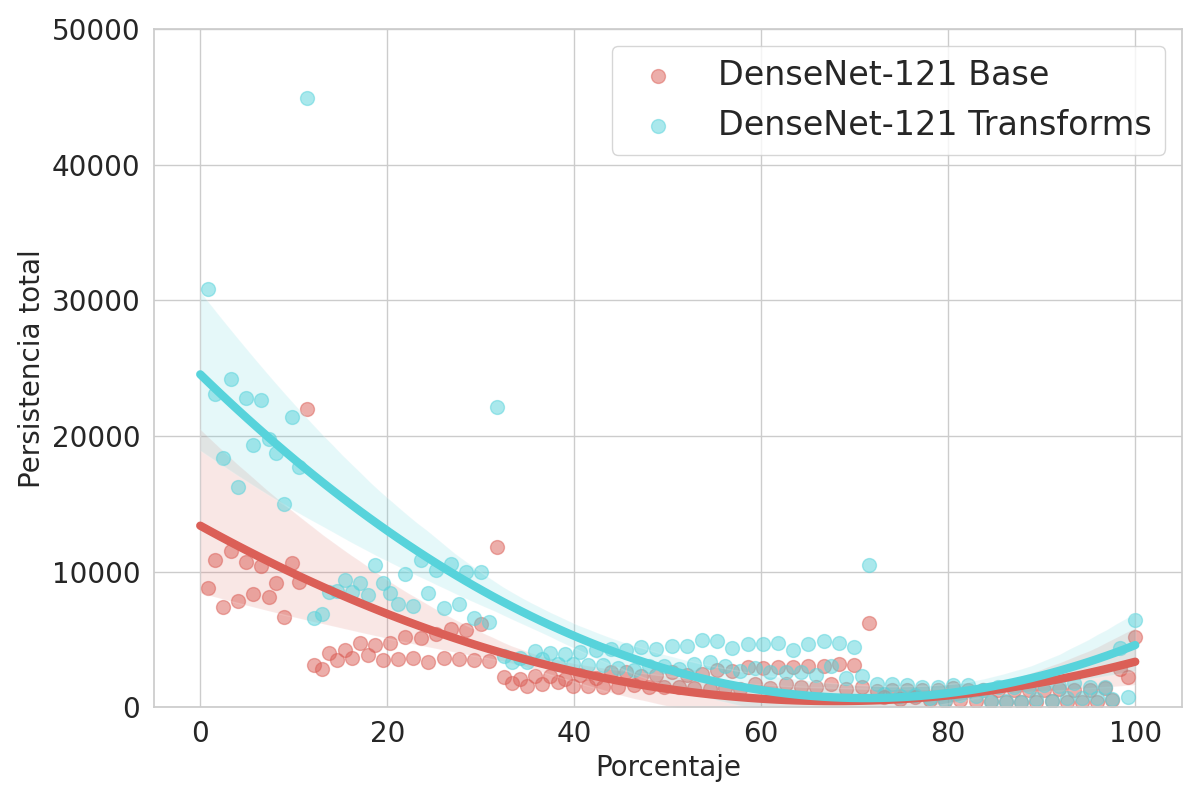
\includegraphics[width=\linewidth]{img/mm.png}
		\caption{Persistencia total según el porcentaje de avance en la red para el
			modelo base entrenado EfficientNet-B0 y su versión con aumento de datos.}
		\label{fig:mm-homology-1}
	\end{subfigure}%
	\begin{subfigure}
		{.5\textwidth}
		\centering
		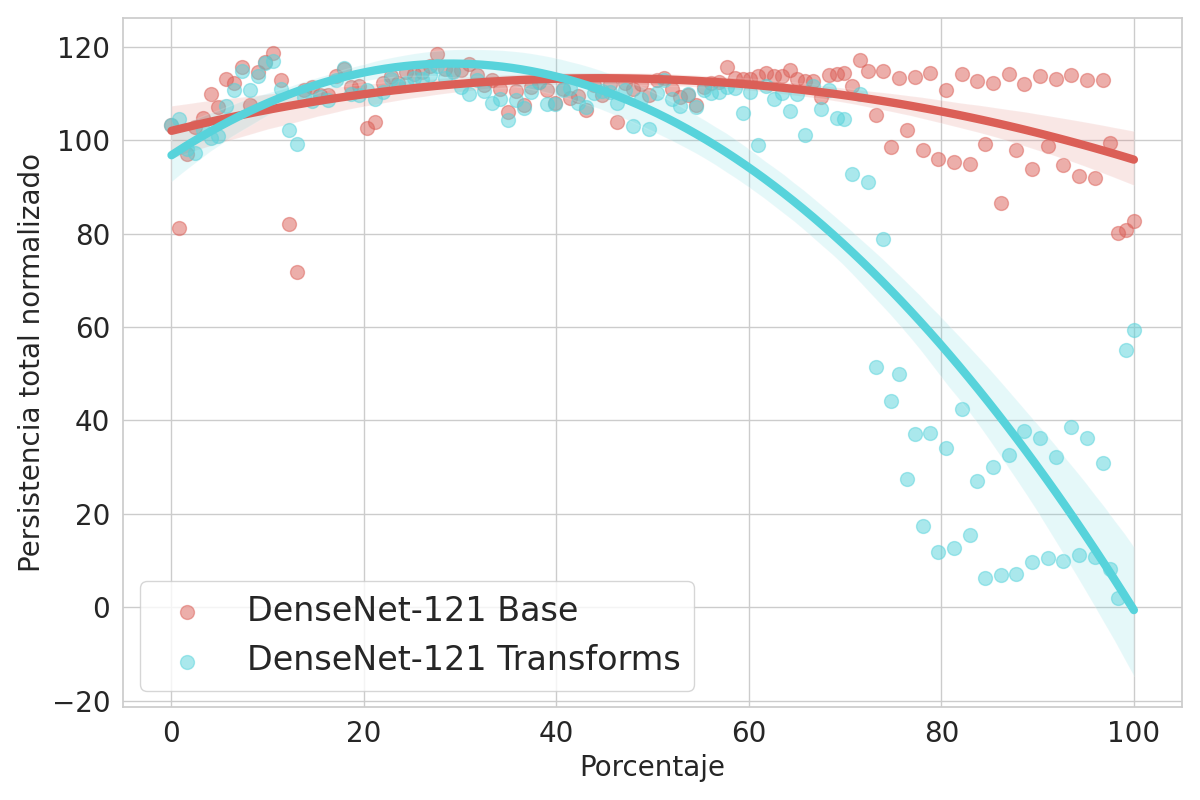
\includegraphics[width=\linewidth]{img/mm_norm.png}
		\caption{Persistencia total normalizada según el porcentaje de avance en la
			red para el modelo base entrenado EfficientNet-B0 y su versión con aumento
			de datos.}
		\label{fig:mm-homology-2}
	\end{subfigure}
	\caption{Comparación de la persistencia total (a) y la persistencia total
		normalizada (b) para EfficientNet-B0 Base y EfficientNet-B0 Transforms en
		función del porcentaje de avance de los datos a través de la red para la
		especificidad Marca-Modelo.}
	\label{fig:mm-homology}
\end{figure}

Los resultados recién vistos muestran patrones interesantes en el comportamiento
del modelo cuando realizamos aumento de datos: tiende a realizar modificaciones más
intensas en fases anteriores de la red y simplificar las estructuras al final del
modelo. Este comportamiento muestra que las componentes conexas al final de la
red son más compactas y están mejor definidas, lo que lleva a una reducción de la
complejidad topológica. No solo eso, si no que al tener en cuenta las clases de persistencia
homológicas de dimensión 1, también se reducen el número de componentes conexas
que forman bucles, lo que evita entrelazamientos entre éstas.

\subsection{Comparación según la granularidad de las clases}
\label{subsec:grano}

\paragraph{EfficientNet-B0}

EfficientNet-B0 ha mostrado el mejor rendimiento en las métricas empleadas para
la especificidad Marca. La persistencia total del modelo entrenado en Marca-Modelo
en la \autoref{fig:efficientnet-1} muestra transformaciones más agresivas en la homología
persistente de los datos. Aquí, en los extremos de la ejecución los datos presentan
una persistencia total más alta y un mínimo inferior al del modelo entrenado para
Marca.

Por su parte, la persistencia total normalizada muestra valores regularmente
superiores para la especificidad Marca-Modelo a los de Marca (\autoref{fig:efficientnet-2}).
Estos hechos parecen coherentes, pues a pesar de corresponderse con el mismo
conjunto de datos, la necesidad de etiquetar una mayor variedad de clases implica
un desglose más fino de las características de los datos y en consecuencia, una
complejidad topológica mayor.

\begin{figure}[H]
	\centering
	\begin{subfigure}
		{.5\textwidth}
		\centering
		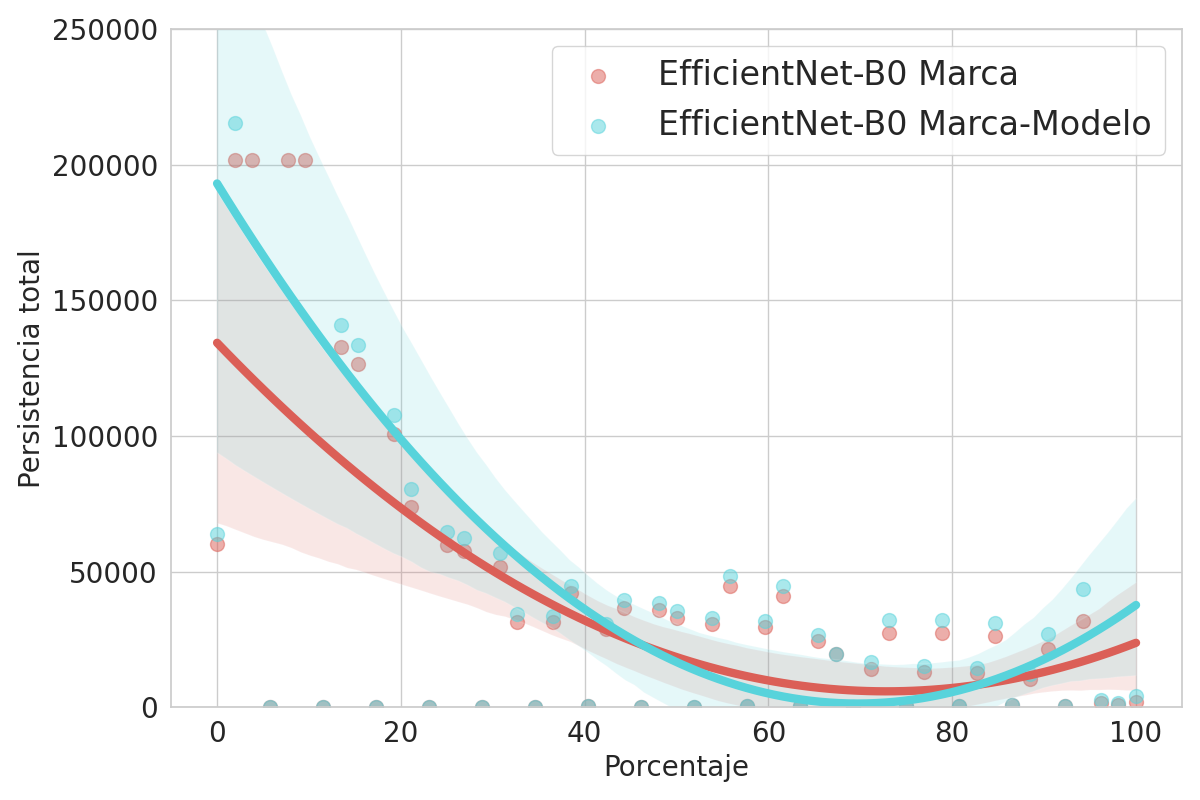
\includegraphics[width=\linewidth]{img/general_efficientnet.png}
		\caption{Persistencia total según el porcentaje de avance en la red para el
			modelo EfficientNet-B0 entrenado para las especificidades Marca y Marca-Modelo.}
		\label{fig:efficientnet-1}
	\end{subfigure}%
	\begin{subfigure}
		{.5\textwidth}
		\centering
		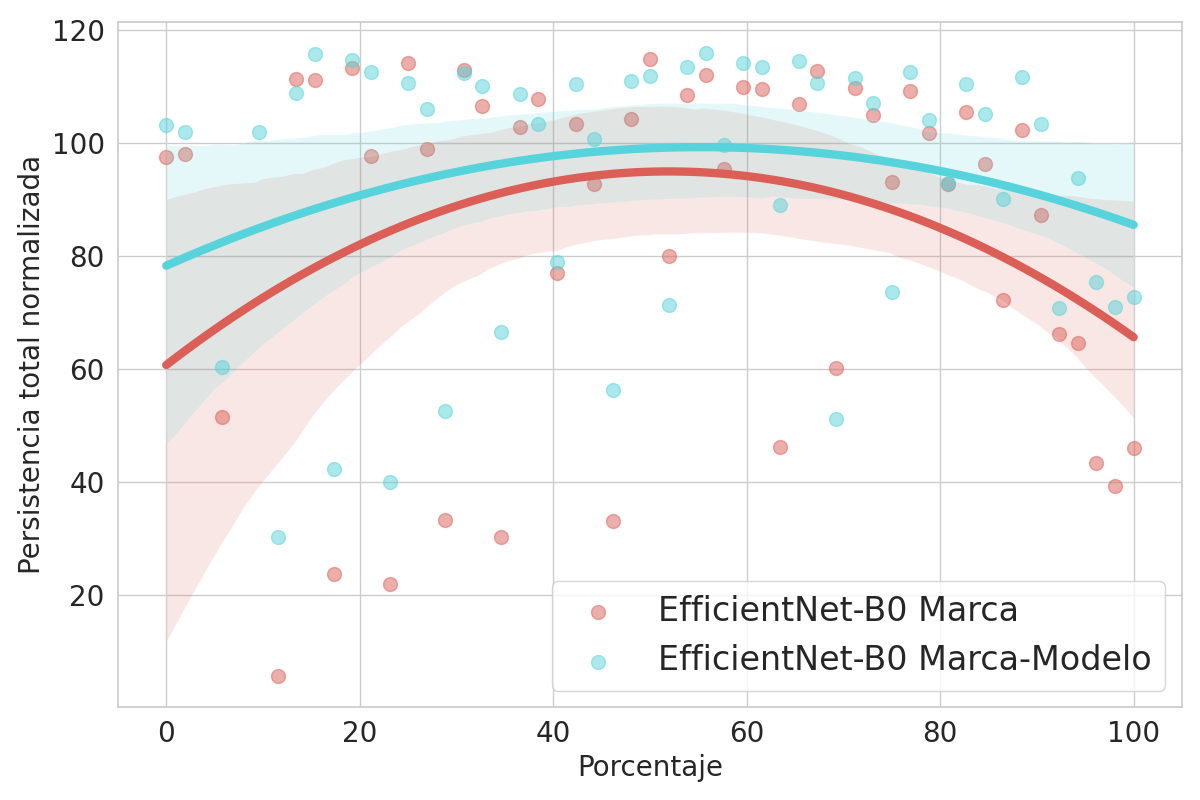
\includegraphics[width=\linewidth]{img/general_efficientnet_norm.png}
		\caption{Persistencia total normalizada según el porcentaje de avance en la
			red para el modelo EfficientNet-B0 entrenado para las especificidades Marca
			y Marca-Modelo.}
		\label{fig:efficientnet-2}
	\end{subfigure}
	\caption{Comparación de la persistencia total (a) y la persistencia total
		normalizada (b) para EfficientNet-B0 entrenado con SGD y un tamaño de lote 64
		en función del porcentaje de avance de los datos a través de la red para las
		especificidades Marca y Marca-Modelo.}
	\label{fig:efficientnet}
\end{figure}

\paragraph{DenseNet-121}

En cuanto a DenseNet-121, vemos en la \autoref{fig:densenet-1} que ambas curvas
se asemejan más que en el caso anterior. Es interesante ver como en el último instante
de la red, el modelo entrenado para la especificidad Marca-Modelo presenta una
subida de persistencia considerable, mientras que la de Marca es más modesta.
Este hecho muestra claramente la necesidad del modelo de deshacer la
simplificación realizada con el fin de separar los datos para la clasificación.

Además, las muestras tomadas en los distintos instantes de la red muestran cuatro
puntos con un aumento considerable de la persistencia total. Estos instantes
coinciden con los puntos donde se encuentran las activaciones de transición
entre los cuatro bloques densos que presenta DenseNet-121, mostrando cómo las conexiones
residuales entre dichos bloques aumenta la complejidad topológica de los datos.

Por otro lado, la \autoref{fig:densenet-2} nos muestra cómo, de nuevo, la
persistencia total normalizada presenta en general valores inferiores para la
especificidad Marca. Otra observación relevante es la reducción de complejidad más
progresiva y gradual que muestra el modelo de Marca en la segunda mitad de la inferencia.
El hecho de que DenseNet-121 entrenado con una mayor granularidad requiera de
mayor persistencia durante más tiempo puede deberse a la clara dificultad
añadida por el aumento de clases.

\begin{figure}[H]
	\centering
	\begin{subfigure}
		{.5\textwidth}
		\centering
		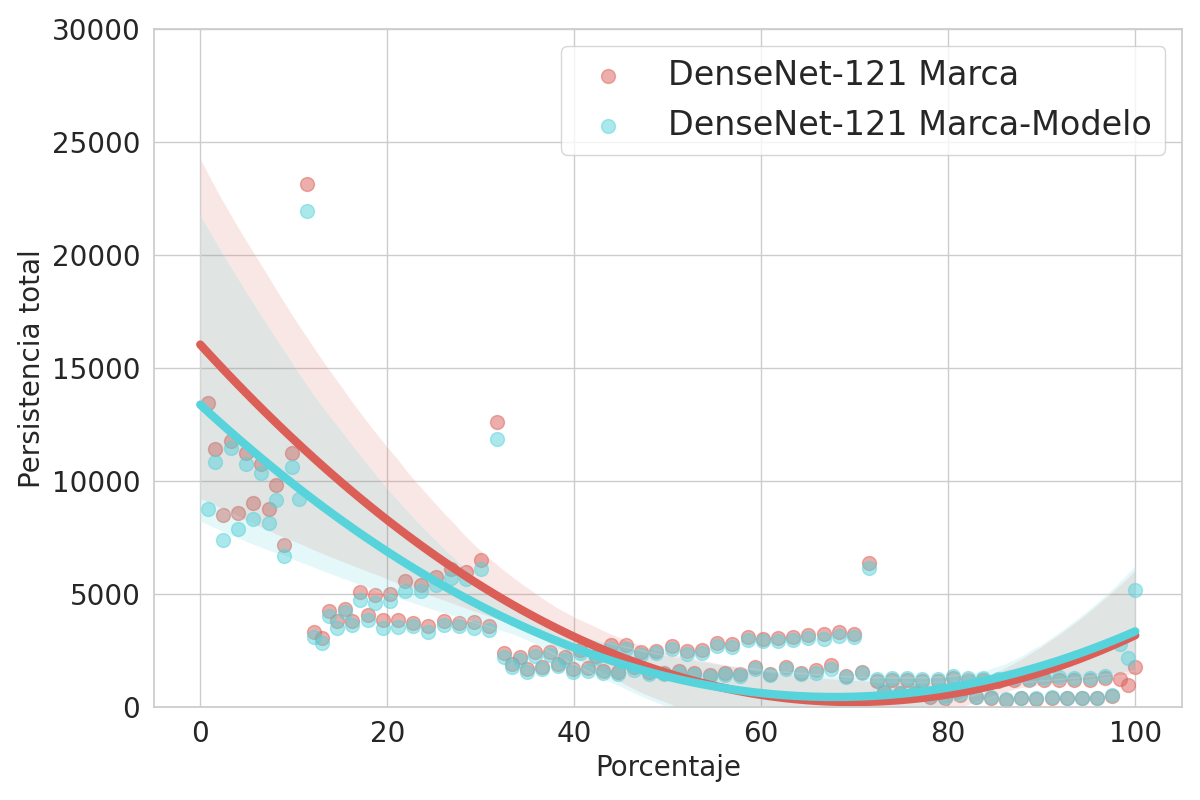
\includegraphics[width=\linewidth]{img/general_densenet.png}
		\caption{Persistencia total según el porcentaje de avance en la red para el
			modelo DenseNet-121 entrenado para las especificidades Marca y Marca-Modelo.}
		\label{fig:densenet-1}
	\end{subfigure}%
	\begin{subfigure}
		{.5\textwidth}
		\centering
		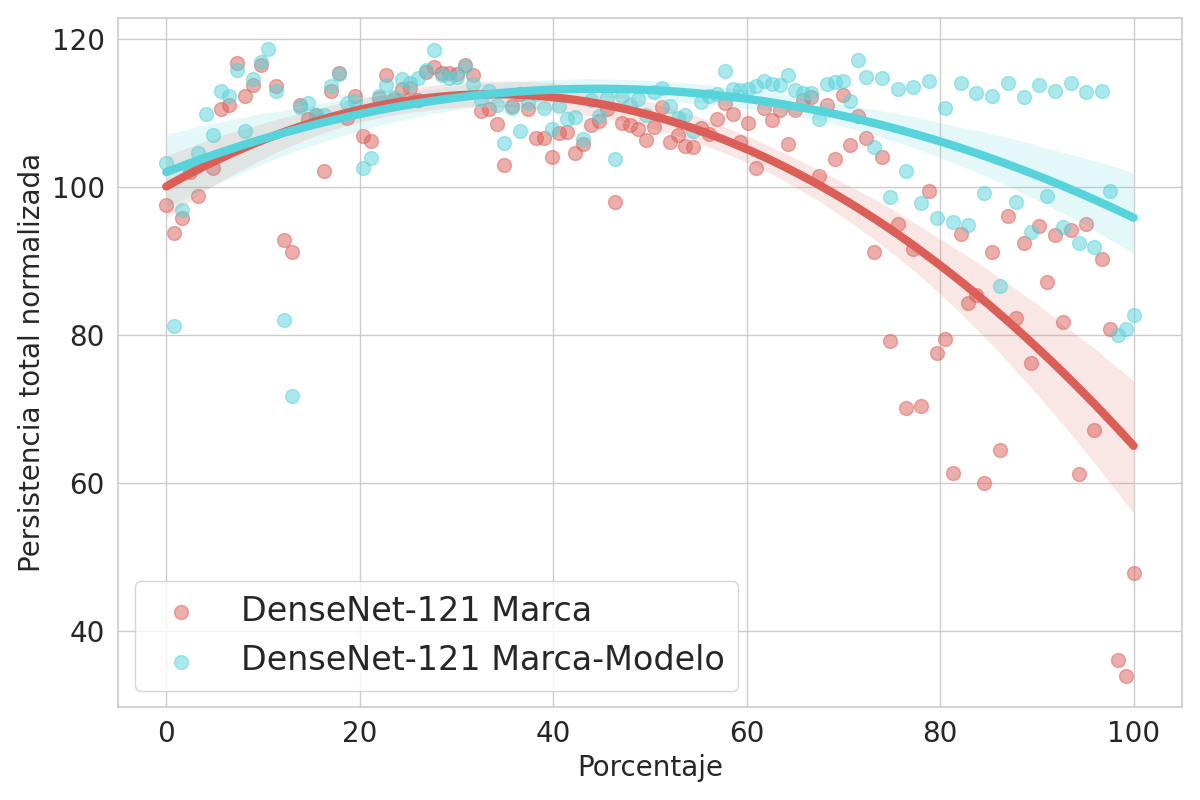
\includegraphics[width=\linewidth]{img/general_densenet_norm.png}
		\caption{Persistencia total normalizada según el porcentaje de avance en la
			red para el modelo DenseNet-121 entrenado para las especificidades Marca y
			Marca-Modelo.}
		\label{fig:densenet-2}
	\end{subfigure}
	\caption{Comparación de la persistencia total (a) y la persistencia total
		normalizada (b) para DenseNet-121 entrenado con SGD y un tamaño de lote 32 en
		función del porcentaje de avance de los datos a través de la red para las
		especificidades Marca y Marca-Modelo.}
	\label{fig:densenet}
\end{figure}

\subsection{Comparación según el subconjunto de datos}
\label{subsec:set}

Hasta ahora hemos estado viendo como distintos modelos con distintos
hiperparámetros y granularidad durante la etapa de entrenamiento afectan a la
variedad subyacente de los datos empleados. A continuación, compararemos cómo
transforma un mismo modelo los propios datos en función del subconjunto al que
pertenecen: entrenamiento, validación y test.

\paragraph{Especificidad Marca: EfficientNet-B0}

Lo primero que observamos en las Figuras \ref{fig:m_set_base} y
\ref{fig:m_set_trans} es una mayor persistencia total al inicio sobre el
conjunto de entrenamiento respecto al de validación y test en ambos modelos. Por
otro lado, en la \autoref{fig:m_set_base}, que muestra los resultados con mejores
métricas, los conjuntos de validación y test muestran una persistencia total
prácticamente idéntica, mientras que el modelo con aumento de datos presenta mayores
discrepancias al respecto.

Por lo que se refiere a la persistencia total normalizada (Figuras
\ref{fig:m_set_base_norm} y \ref{fig:m_set_trans_norm}), observamos tendencias
muy similares, donde las curvas de validación y test muestran un ajuste más fino
al de entrenamiento para el modelo base que para el modelo con aumento de datos.

\begin{figure}[H]
	\centering
	\begin{subfigure}
		{.45\textwidth}
		\centering
		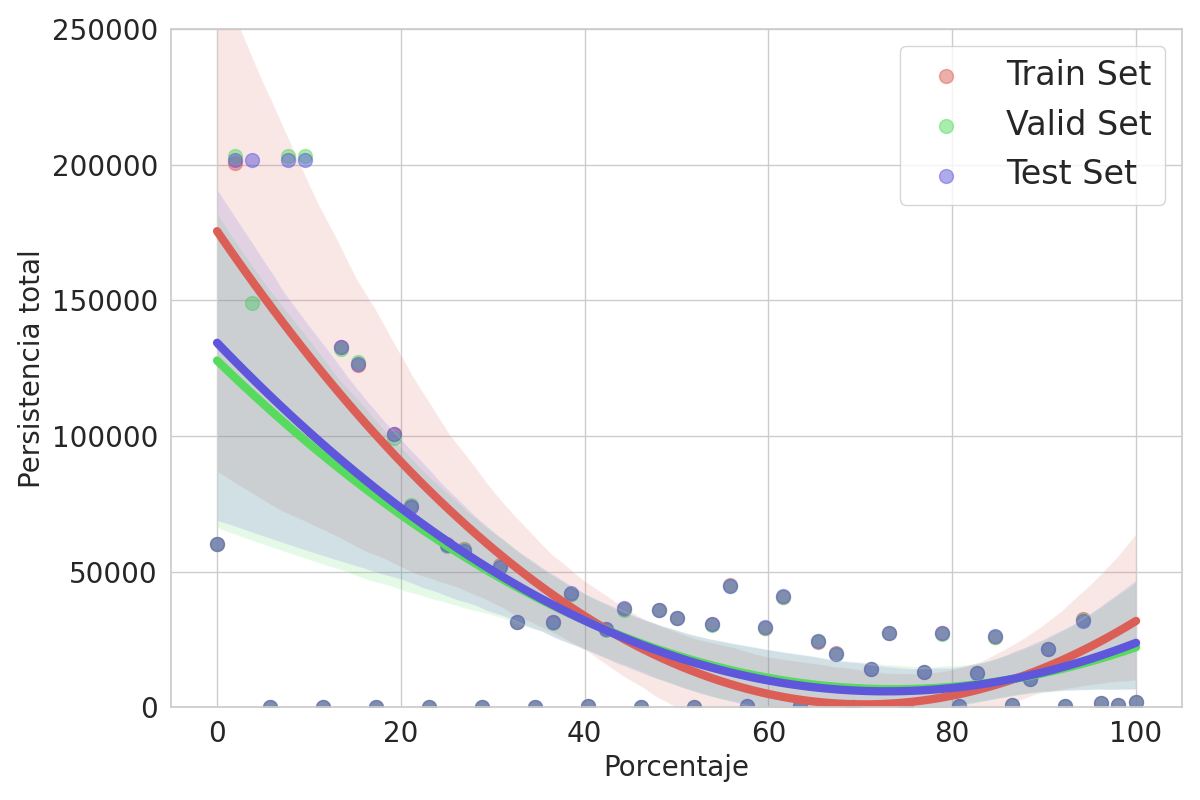
\includegraphics[width=\linewidth]{img/m_set_base.png}
		\caption{Persistencia total según el porcentaje de avance en la red para los
			conjuntos de entrenamiento, validación y test.}
		\label{fig:m_set_base}
	\end{subfigure}
	\begin{subfigure}
		{.45\textwidth}
		\centering
		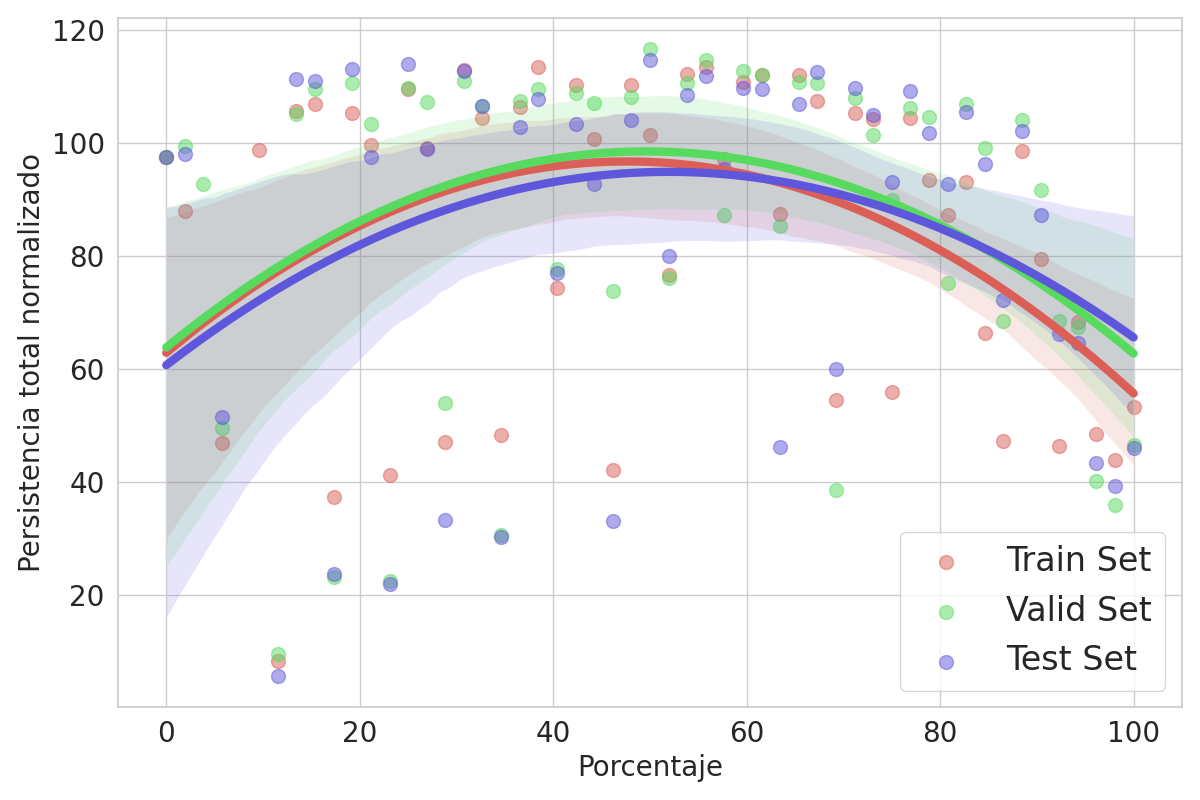
\includegraphics[width=\linewidth]{img/m_set_base_norm.png}
		\caption{Persistencia total normalizada según el porcentaje de avance en la
			red para los conjuntos de entrenamiento, validación y test.}
		\label{fig:m_set_base_norm}
	\end{subfigure}
	\begin{subfigure}
		{.45\textwidth}
		\centering
		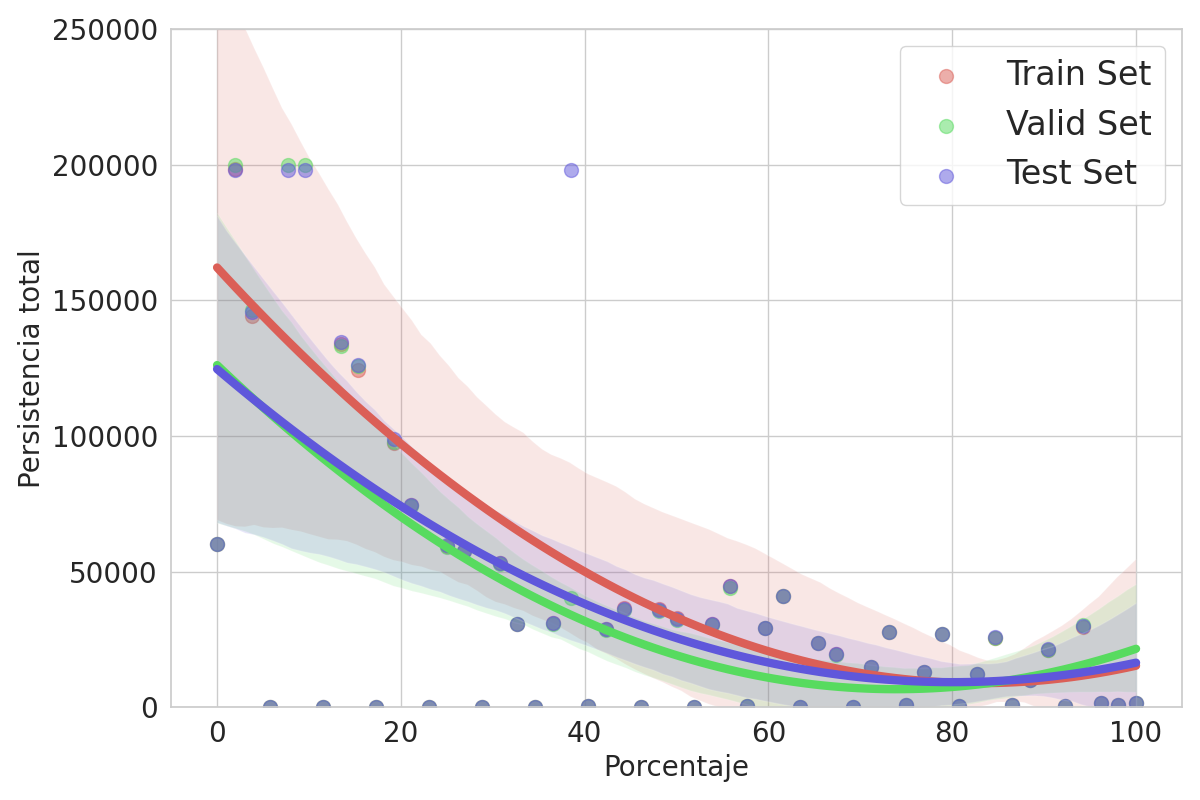
\includegraphics[width=\linewidth]{img/m_set_trans.png}
		\caption{Persistencia total según el porcentaje de avance en la red con
			aumento de datos para los conjuntos de entrenamiento, validación y test.}
		\label{fig:m_set_trans}
	\end{subfigure}%
	\begin{subfigure}
		{.45\textwidth}
		\centering
		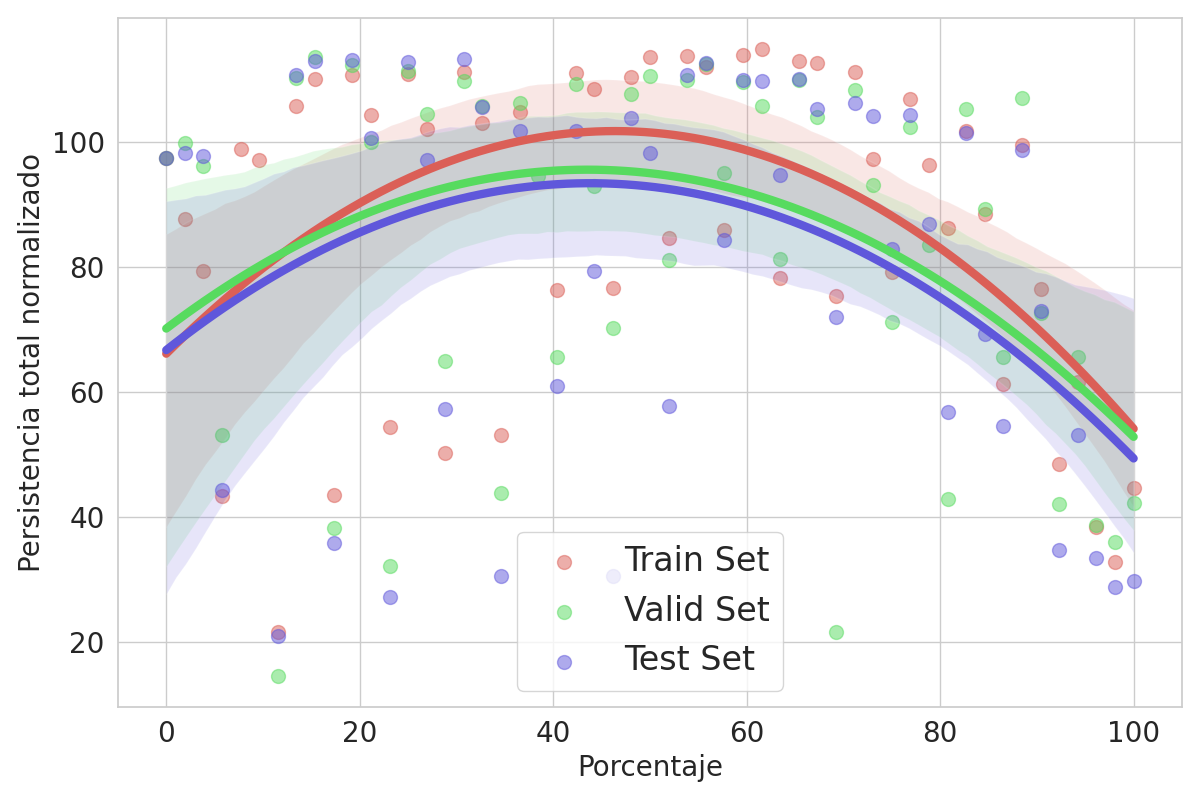
\includegraphics[width=\linewidth]{img/m_set_trans_norm.png}
		\caption{Persistencia total normalizada según el porcentaje de avance en la
			red con aumento de datos para los conjuntos de entrenamiento, validación y test.}
		\label{fig:m_set_trans_norm}
	\end{subfigure}
	\caption{Comparación de la persistencia total (a, c) y la persistencia total normalizada
		(b, d) para los conjuntos de entrenamiento, validación y test para la especificidad
		Marca. Las Figuras (a) y (b) representan el modelo base, mientras que las Figuras
		(c) y (d) representan el modelo con aumento de datos.}
	\label{fig:m-set}
\end{figure}

\paragraph{Especificidad Marca-Modelo: DenseNet-121}

Las Figuras \ref{fig:mm_set_base} y \ref{fig:mm_set_trans} muestran un ajuste de
la persistencia total prácticamente perfecto entre los tres subconjuntos de
datos. Más aún, podemos ver cómo el modelo que ha presentado mejores métricas en
el conjunto de test, es decir, el modelo con aumento de datos, presenta un ajuste
mucho más fino entre los valores de persistencia total normalizados para los tres
subconjuntos (\autoref{fig:mm_set_trans_norm}). Es interesante observar como en
esta ocasión, los puntos obtenidos se comportan de manera más homogénea independientemente
del subconjunto escogido, a diferencia de lo observado en la
\autoref{fig:mm_set_base_norm}.

\begin{figure}[H]
	\centering
	\begin{subfigure}
		{.45\textwidth}
		\centering
		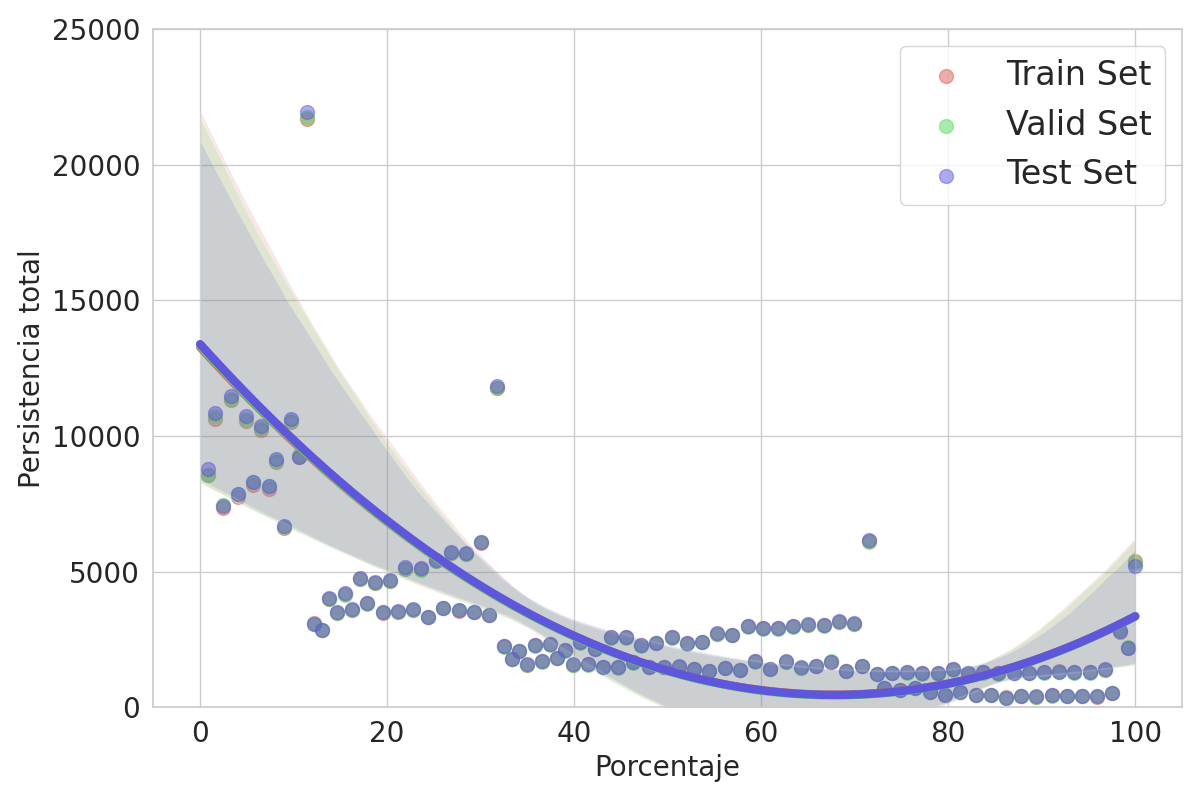
\includegraphics[width=\linewidth]{img/mm_set_base.png}
		\caption{Persistencia total según el porcentaje de avance en la red para los
			conjuntos de entrenamiento, validación y test.}
		\label{fig:mm_set_base}
	\end{subfigure}
	\begin{subfigure}
		{.45\textwidth}
		\centering
		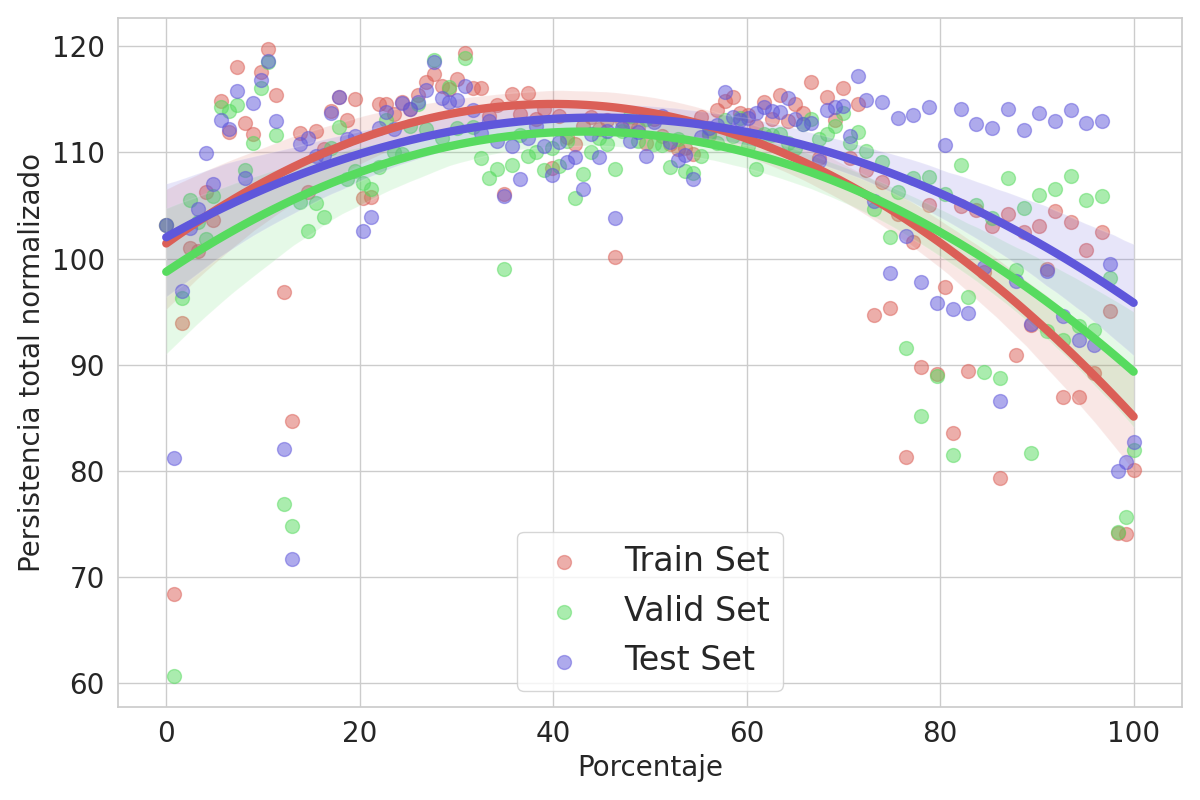
\includegraphics[width=\linewidth]{img/mm_set_base_norm.png}
		\caption{Persistencia total normalizada según el porcentaje de avance en la
			red para los conjuntos de entrenamiento, validación y test.}
		\label{fig:mm_set_base_norm}
	\end{subfigure}
	\begin{subfigure}
		{.45\textwidth}
		\centering
		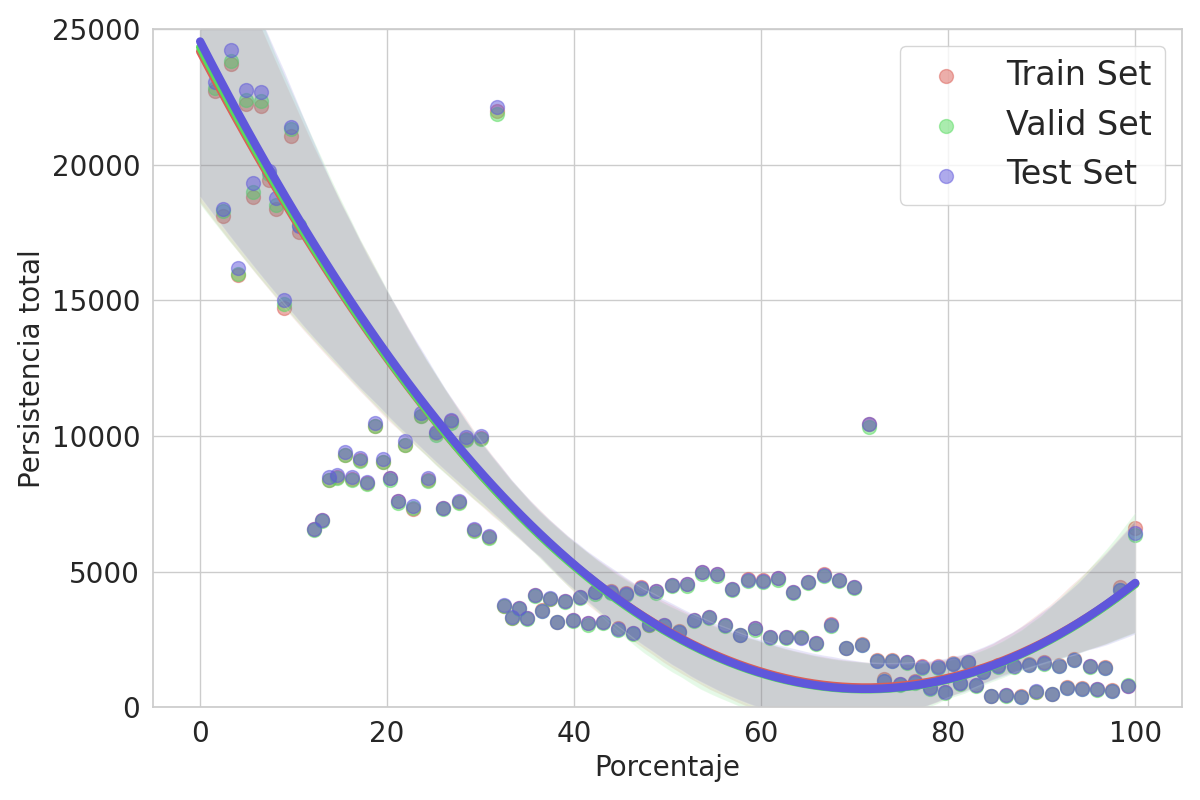
\includegraphics[width=\linewidth]{img/mm_set_trans.png}
		\caption{Persistencia total según el porcentaje de avance en la red con
			aumento de datos para los conjuntos de entrenamiento, validación y test.}
		\label{fig:mm_set_trans}
	\end{subfigure}%
	\begin{subfigure}
		{.45\textwidth}
		\centering
		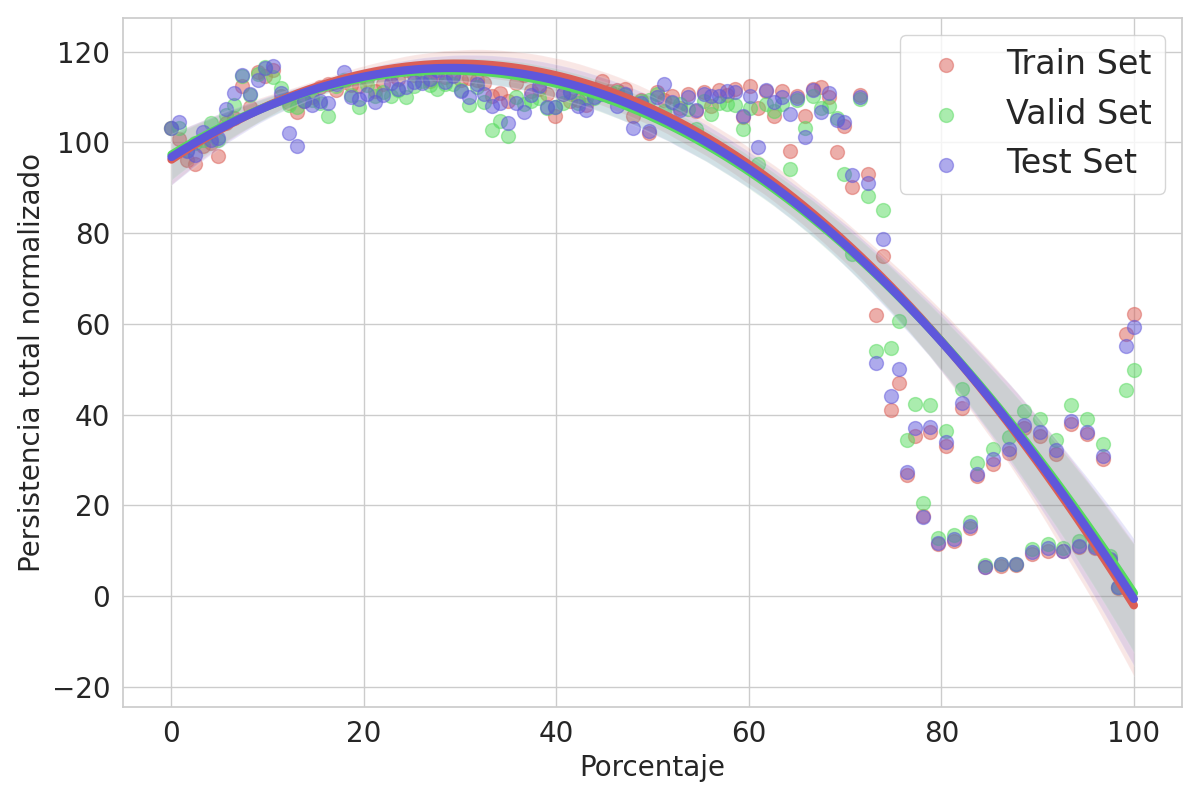
\includegraphics[width=\linewidth]{img/mm_set_trans_norm.png}
		\caption{Persistencia total normalizada según el porcentaje de avance en la
			red con aumento de datos para los conjuntos de entrenamiento, validación y test.}
		\label{fig:mm_set_trans_norm}
	\end{subfigure}
	\caption{Comparación de la persistencia total (a, c) y la persistencia total normalizada
		(b, d) para los conjuntos de entrenamiento, validación y test para la especificidad
		Marca-Modelo. Las Figuras (a) y (b) representan el modelo base, mientras que las
		Figuras (c) y (d) representan el modelo con aumento de datos.}
	\label{fig:mm-set}
\end{figure}

Las Figuras \ref{fig:m-set} y \ref{fig:mm-set} muestran cómo las redes mejor entrenadas
obtienen una coincidencia mayor entre los distintos subconjuntos de datos empleados
típicamente en el entrenamiento de las CNNs, lo que indica un mejor aprendizaje
de la variedad subyacente de la que parten los datos.

\subsection{Reflexiones sobre la topología en CNNs}

El análisis recién realizado sobre cómo diferentes configuraciones de modelos de
CNNs afectan las características topológicas de los datos ha mostrado patrones claros.
Las arquitecturas estudiadas comienzan simplificando los datos, probablemente como
consecuencia de los cambios de la dimensionalidad de las activaciones y para eliminar
ruido o detalles innecesarios. Sin embargo, hacia el final del proceso de aprendizaje,
la persistencia total aumenta nuevamente. Esta dinámica parece ser una estrategia
para crear representaciones más ricas y detalladas que ayuden a diferenciar mejor
entre las clases durante la clasificación de instancias.

El tipo de optimizador utilizado, como Adam o SGD, también juega un papel relevante,
pero su impacto varía a lo largo del entrenamiento. Adam, que ajusta
dinámicamente las tasas de aprendizaje, parece ser especialmente efectivo en las
fases iniciales, facilitando una rápida reducción de la persistencia total. En cambio,
SGD adopta un enfoque diferente, partiendo de una mayor complejidad y realizando
transformaciones más agresivas en la topología de los datos.

Sorprendentemente, el tamaño del lote mostró tener un impacto mínimo en la
homología persistente. Esto indica que los ajustes en la topología de los datos son
bastante robustos a variaciones en el tamaño del lote, siendo este un factor a
tener en cuenta a la hora de trabajar con la topología de los datos.

El aumento de datos es otro factor importante. Al entrenar modelos con una mayor
variedad de datos durante el entrenamiento, se promueve una adaptación más
temprana y efectiva a la complejidad relativa de los datos, lo que lleva a una menor
necesidad de trabajar los datos de manera tan intensiva en etapas posteriores.
Esto no solo ayuda a generalizar mejor sino también a simplificar eficazmente
esa complejidad hacia el final del entrenamiento, preparando el modelo para tareas
de clasificación más precisas.

La granularidad en la clasificación necesita que los modelos manejen y preserven
una complejidad topológica mayor durante más tiempo, manteniendo las
distinciones claras entre múltiples categorías. Al comparar cómo se comportan los
modelos en diferentes subconjuntos de datos, es notable que aquellos con mejores
métricas ajustan más precisamente sus características topológicas entre los
conjuntos de entrenamiento, validación y prueba, mostrando un aprendizaje más
consistente y profundo de la estructura subyacente de los datos.

\section{Propuesta de mejora: regularización topológica}
\label{subsec:proposal}

El análisis realizado sobre la homología persistente de los datos ha mostrado ciertos
patrones y resultados que podrían aprovecharse durante el entrenamiento de las CNNs.
En esta sección aplicamos las propuestas realizadas con el fin de confirmar
nuestras hipótesis y hallar nuevas técnicas que mejoren y faciliten el
aprendizaje a las CNNs.

\subsection{Mejora en clasificación}

\paragraph{Especificidad Marca: EfficientNet-B0}

La propuesta de emplear el regularizador topológico para mejorar la tasa de clasificación
en EfficientNet-B0 parece haber mostrado una leve mejoría respecto al modelo base
y el modelo refinado sin emplear el regularizador (\autoref{tab:efficientnet-refined}).

\begin{table}[H]
	\centering
	\begin{adjustbox}
		{width=0.8\textwidth}
		\begin{tabular}{|c|c|c|c|c|c|}
			\hline
			\textbf{Modelo}          & $\alpha$ & \textbf{Exactitud} & \textbf{Precisión} & \textbf{Sensibilidad} & \textbf{F1-Score} \\
			\hline
			EfficientNet-B0 Base     & -        & 0.9505             & 0.9462             & 0.9386                & 0.9423            \\
			\hline
			EfficientNet-B0 Refinado & 0.0      & 0.9598             & 0.9512             & 0.9445                & 0.9478            \\
			\hline
			EfficientNet-B0 Refinado & 0.001    & 0.9598             & 0.9496             & 0.9448                & 0.9472            \\
			\hline
			EfficientNet-B0 Refinado & 0.005    & \textbf{0.9659}    & \textbf{0.9545}    & \textbf{0.9514}       & \textbf{0.9529}   \\
			\hline
			EfficientNet-B0 Refinado & 0.01     & 0.9598             & 0.9517             & 0.9481                & 0.9499            \\
			\hline
			EfficientNet-B0 Refinado & 0.05     & 0.9536             & 0.9515             & 0.9412                & 0.9462            \\
			\hline
			EfficientNet-B0 Refinado & 0.1      & 0.9567             & 0.9475             & 0.9413                & 0.9444            \\
			\hline
			EfficientNet-B0 Refinado & 0.5      & 0.9505             & 0.9486             & 0.9369                & 0.9426            \\
			\hline
			EfficientNet-B0 Refinado & 1.0      & 0.9505             & 0.9453             & 0.9413                & 0.9432            \\
			\hline
		\end{tabular}
	\end{adjustbox}
	\caption{Comparación de métricas tras un proceso de refinamiento en la misma
		especificidad Marca para distintos valores de $\alpha$ en el término de
		regularización del modelo EfficientNet-B0.}
	\label{tab:efficientnet-refined}
\end{table}

Observando la \autoref{fig:efficientnet-refine-1} vemos que la persistencia
total del modelo refinado sin regularizador es generalmente inferior a la del
modelo regularizado. Sin embargo, en las etapas finales muestra un leve repunte
frente al modelo sin regularizar. La persistencia total normalizada sigue mostrando
un comportamiento similar en ambos modelos, siendo algo inferior en la salida
del modelo regularizado (\autoref{fig:efficientnet-refine-2}) .

\begin{figure}[H]
	\centering
	\begin{subfigure}
		{.5\textwidth}
		\centering
		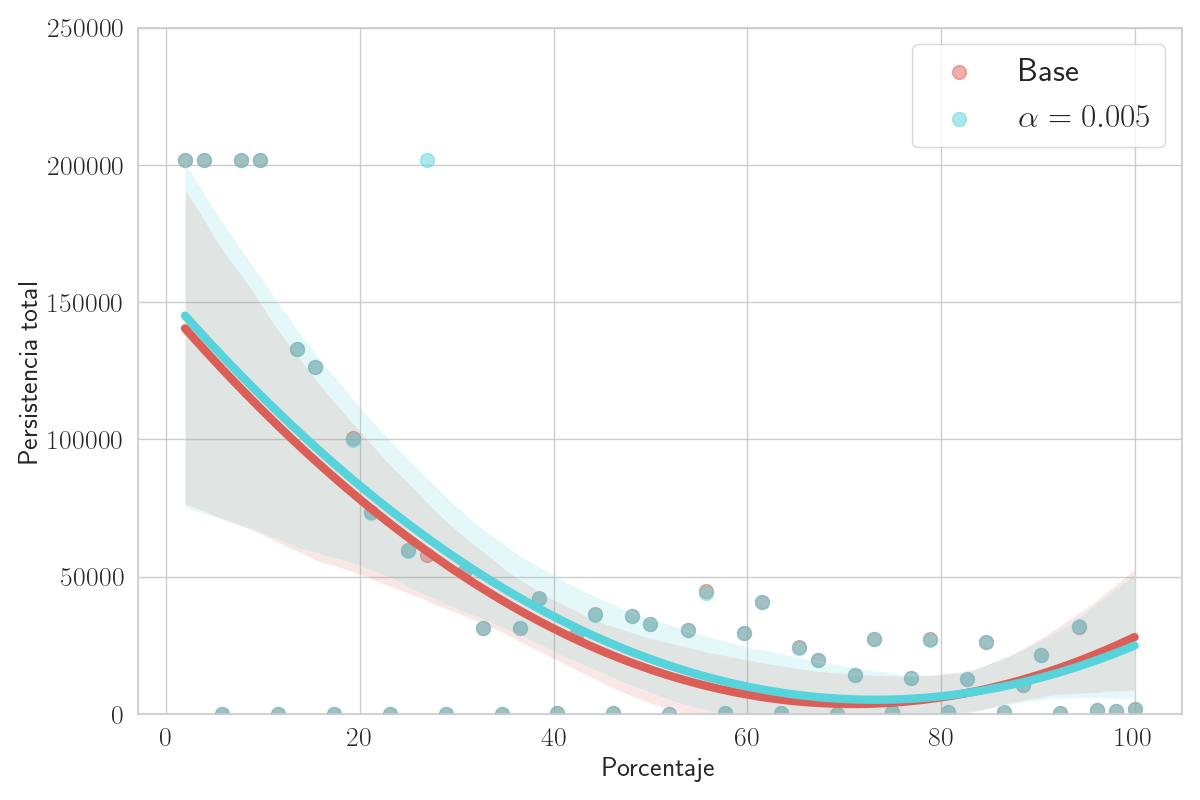
\includegraphics[width=\linewidth]{img/exp_refine_efficientnet.png}
		\caption{Persistencia total según el porcentaje de avance en la red para el
			modelo EfficientNet-B0 refinado para la especificidad Marca.}
		\label{fig:efficientnet-refine-1}
	\end{subfigure}%
	\begin{subfigure}
		{.5\textwidth}
		\centering
		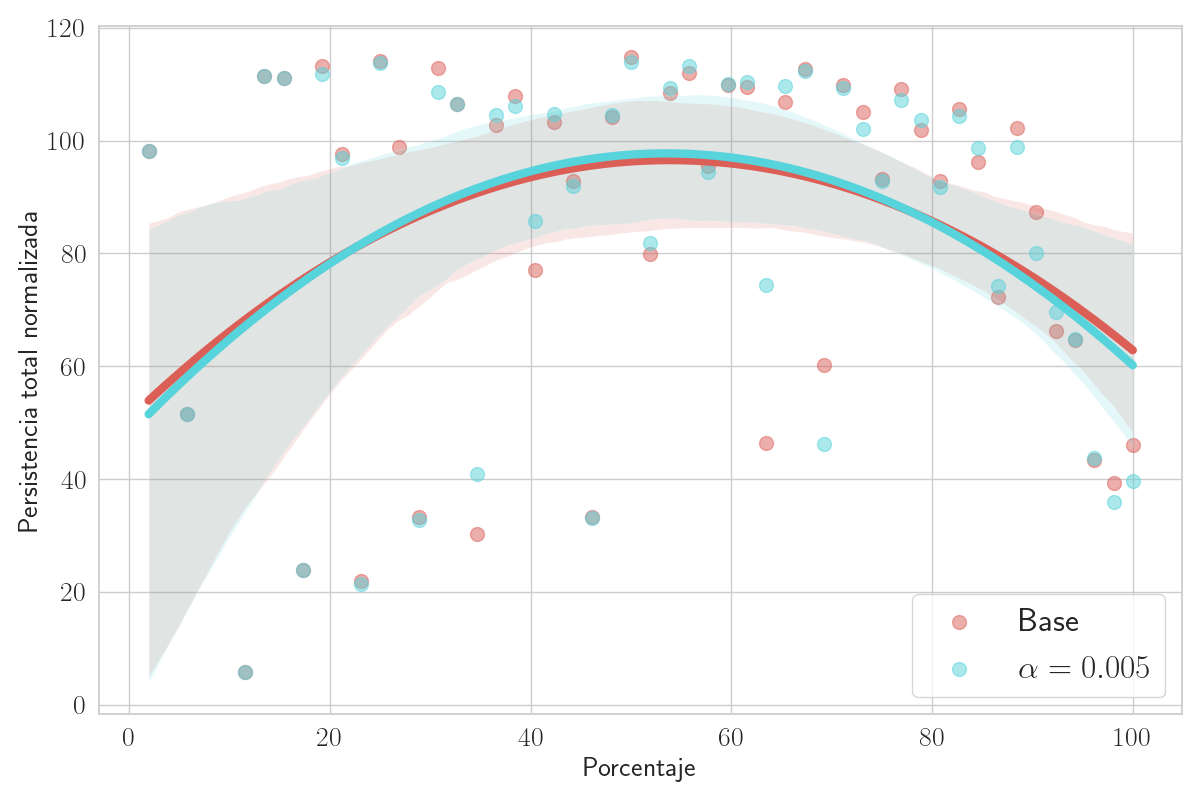
\includegraphics[width=\linewidth]{img/exp_refine_efficientnet_norm.png}
		\caption{Persistencia total normalizada según el porcentaje de avance en la
			red para el modelo EfficientNet-B0 refinado para Marca.}
		\label{fig:efficientnet-refine-2}
	\end{subfigure}
	\caption{Comparación de la persistencia total (a) y la persistencia total
		normalizada (b) para EfficientNet-B0 refinado con SGD y un tamaño de lote 64
		en función del porcentaje de avance de los datos a través de la red para las
		especificidad Marca con y sin regularizador.}
	\label{fig:efficientnet-refine}
\end{figure}

El ejemplo que se ve en la \autoref{fig:ex-efficientnet-refine} muestra la
diferencia entre las activaciones en ambas versiones. En la versión regularizada
desaparecen ciertas activaciones pequeñas para centrarse principalmente en el logo
del coche.

\begin{figure}[H]
	\centering
	\begin{subfigure}
		{.45\textwidth}
		\centering
		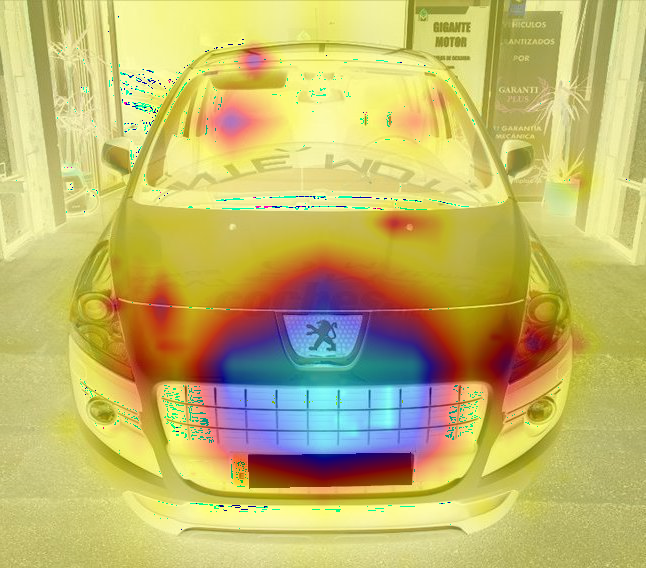
\includegraphics[width=\linewidth]{img/192_false.png}
		\caption{Ejemplo mal clasificado para el modelo EfficientNet-B0 refinado
			para la especificidad Marca.}
		\label{fig:ex-efficientnet-refine-1}
	\end{subfigure}%
	\qquad
	\begin{subfigure}
		{.45\textwidth}
		\centering
		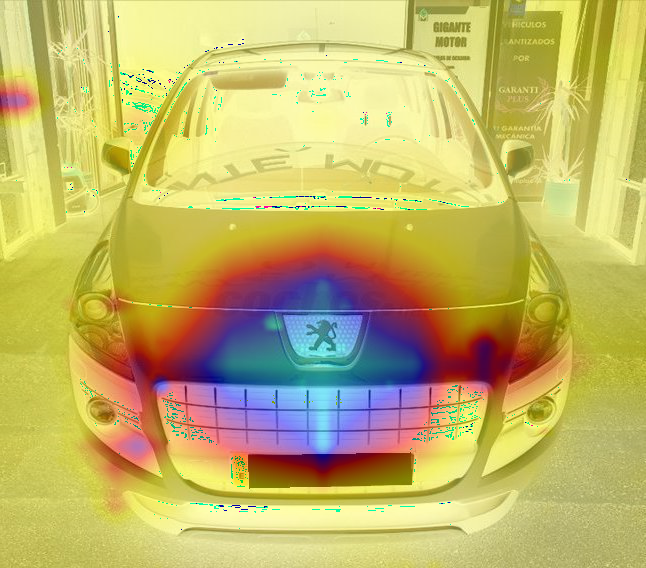
\includegraphics[width=\linewidth]{img/192_true.png}
		\caption{Ejemplo bien clasificado para el modelo EfficientNet-B0 refinado
			con regularización para Marca.}
		\label{fig:ex-efficientnet-refine-2}
	\end{subfigure}
	\caption{Comparación de clasificación para el caso sin regularizar (a) frente
		al regularizado (b) para EfficientNet-B0.}
	\label{fig:ex-efficientnet-refine}
\end{figure}

Es interesante ver cómo pese a la gran similaridad que presentan ambas
alternativas en sus código de barras, pequeñas diferencias logran marcar la diferencia
(\autoref{fig:efficientnet-refine-bc}). Estos detalles son más notables al 100\%
de la ejecución, donde el modelo regularizado topológicamente muestra intervalos
de persistencia de dimensión 1 más cortos.

\paragraph{Especificidad Marca-Modelo: DenseNet-121}

Las observaciones recién realizadas sobre los valores de las métricas se repiten
con mayor fuerza para DenseNet-121 en Marca-Modelo (\autoref{tab:densenet-refine}).
Esta aportación, para el caso donde $\alpha = 0.1$, lleva a una mejora por encima
del 2\% en la exactitud del modelo, mientras que F1-Score llega a aumentar hasta
un 3\% sobre el modelo base. No sólo eso, sino que estos valores superan a los
obtenidos a los del modelo refinado sin el término de regularización, mostrando su
eficacia.

\begin{table}[h]
	\centering
	\begin{adjustbox}
		{width=0.8\textwidth}
		\begin{tabular}{|c|c|c|c|c|c|}
			\hline
			\textbf{Modelo}       & $\alpha$ & \textbf{Exactitud} & \textbf{Precisión} & \textbf{Sensibilidad} & \textbf{F1-Score} \\
			\hline
			DenseNet-121 Base     & -        & 0.9185             & 0.9077             & 0.9126                & 0.9101            \\
			\hline
			DenseNet-121 Refinado & 0.0      & 0.9333             & 0.9220             & 0.9286                & 0.9253            \\
			\hline
			DenseNet-121 Refinado & 0.001    & 0.9333             & 0.9220             & 0.9286                & 0.9253            \\
			\hline
			DenseNet-121 Refinado & 0.005    & 0.9370             & 0.9269             & 0.9336                & 0.9302            \\
			\hline
			DenseNet-121 Refinado & 0.01     & 0.9333             & 0.9220             & 0.9286                & 0.9253            \\
			\hline
			DenseNet-121 Refinado & 0.05     & 0.9370             & 0.9284             & 0.9334                & 0.9308            \\
			\hline
			DenseNet-121 Refinado & 0.1      & \textbf{0.9407}    & \textbf{0.9384}    & \textbf{0.9414}       & \textbf{0.9399}   \\
			\hline
			DenseNet-121 Refinado & 0.5      & 0.9370             & 0.9297             & 0.9330                & 0.9313            \\
			\hline
			DenseNet-121 Refinado & 1.0      & 0.9000             & 0.8997             & 0.8945                & 0.8970            \\
			\hline
		\end{tabular}
	\end{adjustbox}
	\caption{Comparación de métricas tras un proceso de refinamiento en la misma
		especificidad Marca-Modelos para distintos valores de $\alpha$ en el término
		de regularización del modelo DenseNet-121.}
	\label{tab:densenet-refine}
\end{table}

\begin{figure}[H]
	\centering
	% First Column
	\begin{subfigure}
		{.5\textwidth}
		\centering
		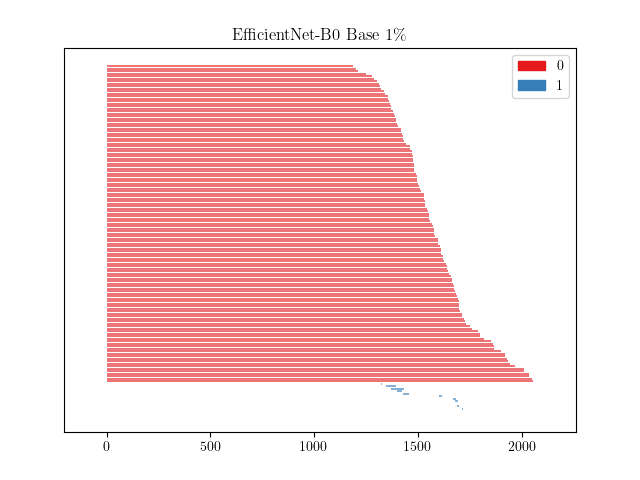
\includegraphics[width=\linewidth]{img/bar_effcientnet_base_0.01.png}
	\end{subfigure}%
	\begin{subfigure}
		{.5\textwidth}
		\centering
		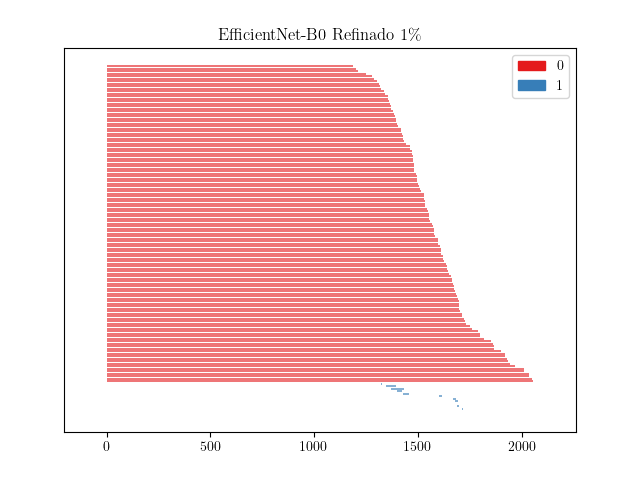
\includegraphics[width=\linewidth]{img/bar_effcientnet_refine_0.01.png}
	\end{subfigure}
	\begin{subfigure}
		{.5\textwidth}
		\centering
		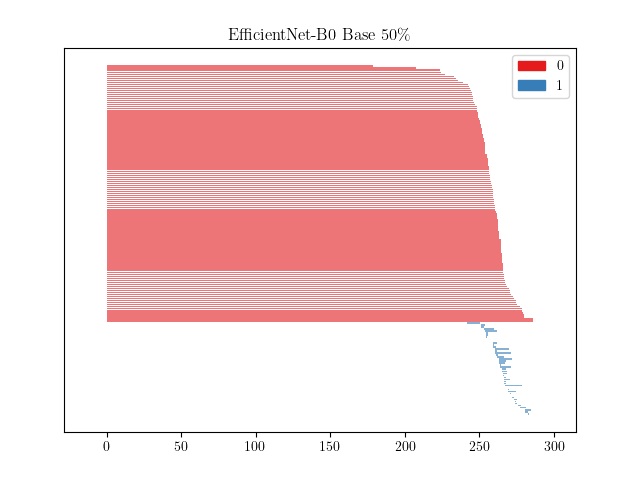
\includegraphics[width=\linewidth]{img/bar_effcientnet_base_0.50.png}
	\end{subfigure}%
	\begin{subfigure}
		{.5\textwidth}
		\centering
		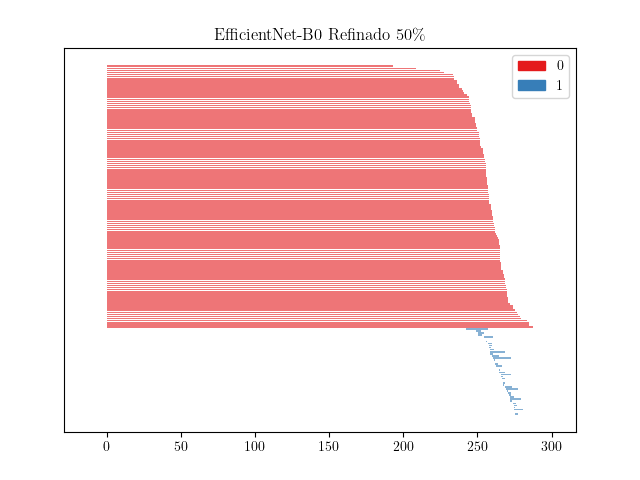
\includegraphics[width=\linewidth]{img/bar_effcientnet_refine_0.50.png}
	\end{subfigure}
	\begin{subfigure}
		{.5\textwidth}
		\centering
		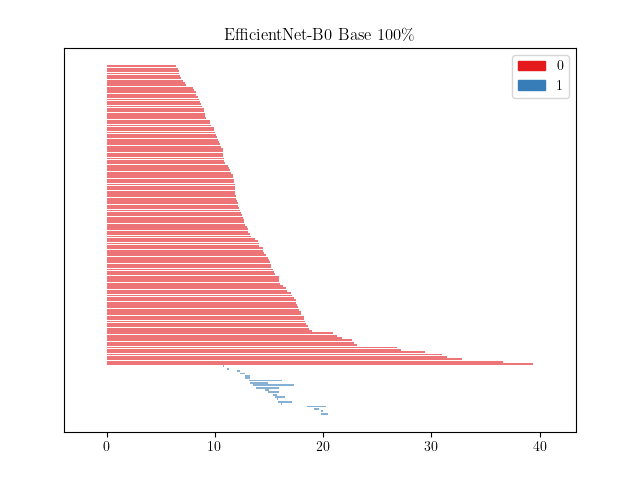
\includegraphics[width=\linewidth]{img/bar_effcientnet_base_1.00.png}
	\end{subfigure}%
	\begin{subfigure}
		{.5\textwidth}
		\centering
		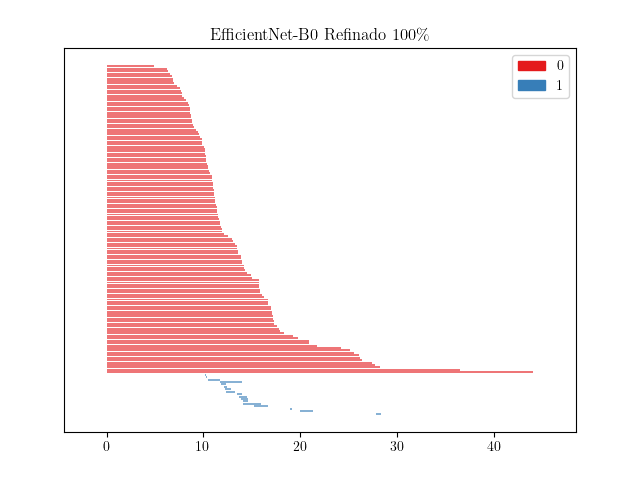
\includegraphics[width=\linewidth]{img/bar_effcientnet_refine_1.00.png}
	\end{subfigure}
	
	\caption{Comparación de los códigos de barras del modelo EfficientNet-B0 para
		el refinamiento en la especificidad Marca sin regularización (izquierda)
		frente al modelo refinado con regularización (derecha). La figura muestra los códigos
		de barras para el conjunto de test tras avanzar un $1\%$ (arriba), un $50\%$ (centro)
		y el $100\%$ (abajo) de la red.}
	\label{fig:efficientnet-refine-bc}
\end{figure}

Las gráficas de persistencia (\autoref{fig:densenet-norm}) apenas muestran diferencias
para ambas versiones, con la excepción de la \autoref{fig:densenet-norm-2}, donde
el modelo regularizado muestra al final del proceso una persistencia total normalizada
ligeramente inferior. Este hecho es especialmente curioso si observamos los
códigos de barras obtenidos en la \autoref{fig:densenet-refine-bc}. Si bien los intervalos
de persistencia son similares a comienzos y mediados de la inferencia, al final
de la red observamos un menor número de componentes conexas persistentes y más
duraderas. Es más, observamos también que aumentan el número y la longitud de
clases de homología persistente de dimensión 1, lo que choca con las hipótesis planteadas.
Un motivo podría deberse a que la importante reducción en el número de
componentes conexas persistentes haya beneficiado más a la reducción de
persistencia total normalizada, de forma que el sacrificio en homología persistente
en dimensión 1 siga siendo una mejor opción en el cómputo total.

\begin{figure}[H]
	\centering
	\begin{subfigure}
		{.5\textwidth}
		\centering
		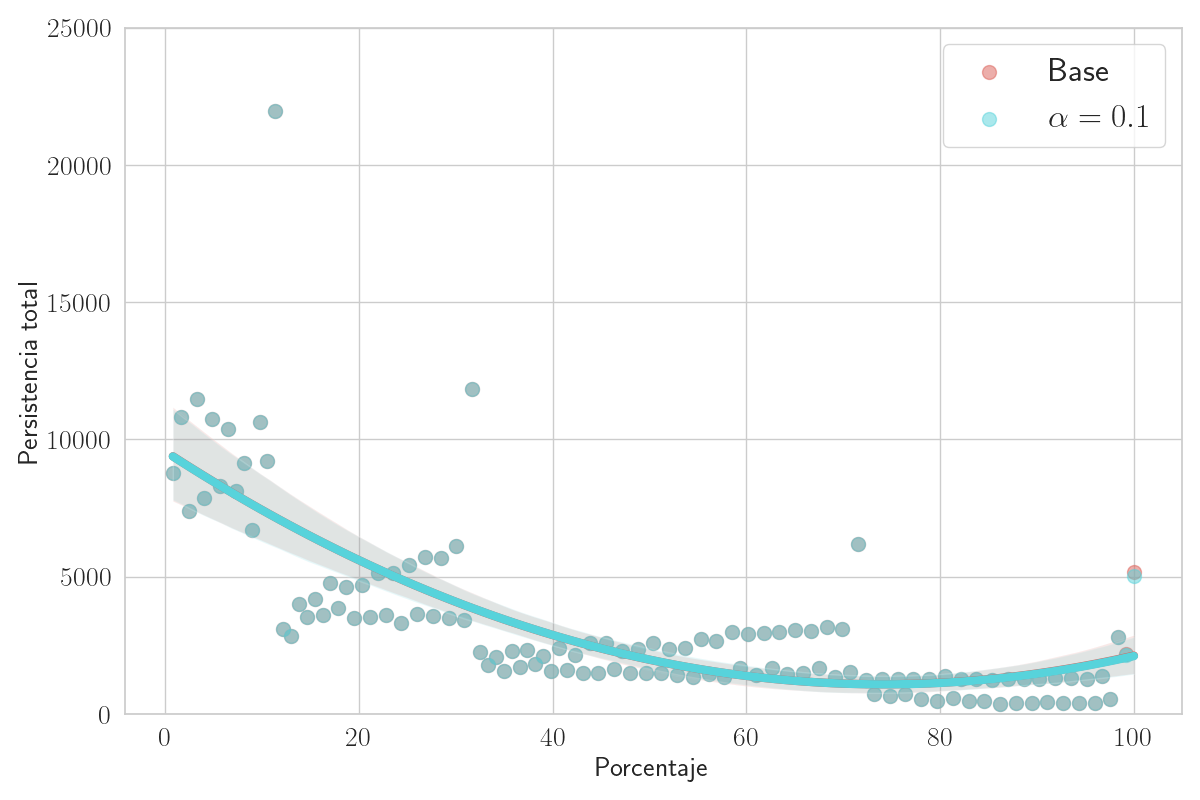
\includegraphics[width=\linewidth]{img/exp_refine_densenet.png}
		\caption{Persistencia total normalizada según el porcentaje de avance en la
			red para el modelo DenseNet-121 refinado para Marca-Modelo.}
		\label{fig:densenet-norm-1}
	\end{subfigure}%
	\begin{subfigure}
		{.5\textwidth}
		\centering
		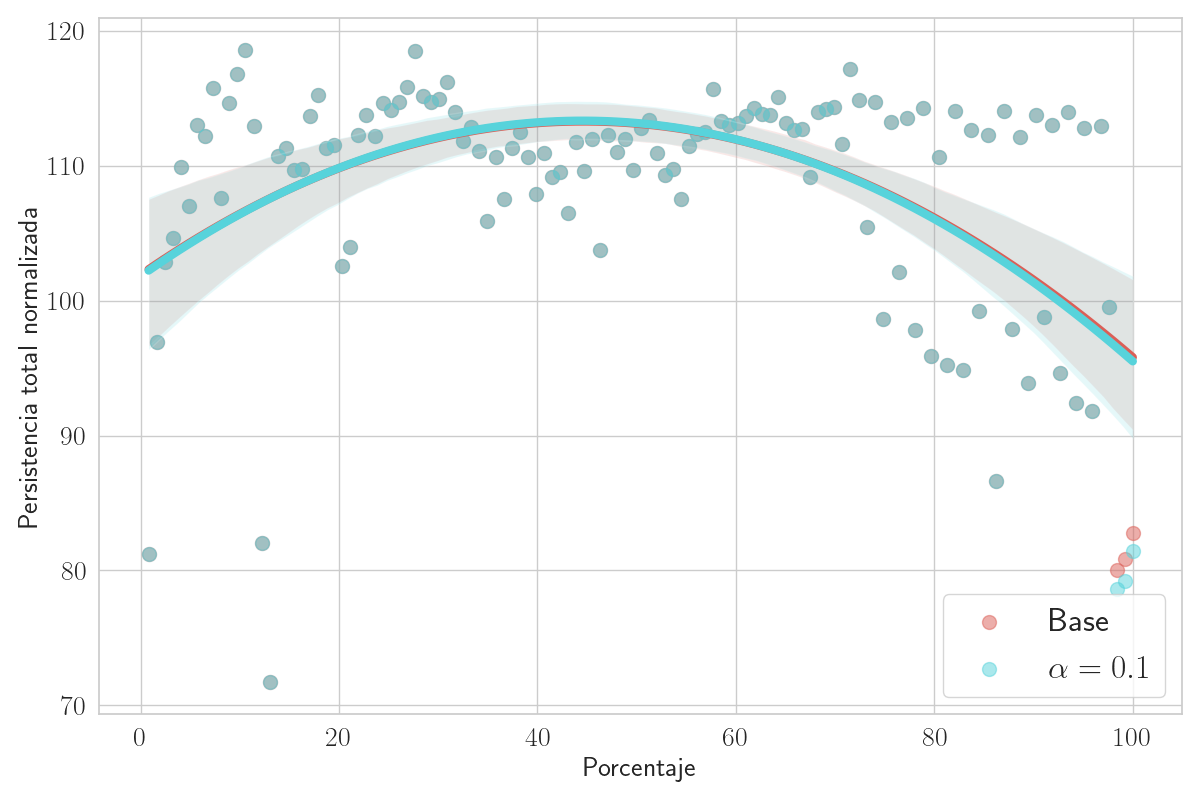
\includegraphics[width=\linewidth]{img/exp_refine_densenet_norm.png}
		\caption{Persistencia total normalizada según el porcentaje de avance en la
			red para el modelo DenseNet-121 refinado para Marca-Modelo.}
		\label{fig:densenet-norm-2}
	\end{subfigure}
	\caption{Comparación de la persistencia total (a) y la persistencia total
		normalizada (b) para DenseNet-121 refinado con SGD y un tamaño de lote 32 en
		función del porcentaje de avance de los datos a través de la red para la
		especificidad Marca-Modelo con y sin regularizador.}
	\label{fig:densenet-norm}
\end{figure}

\begin{figure}[H]
	\centering
	\begin{subfigure}
		{.45\textwidth}
		\centering
		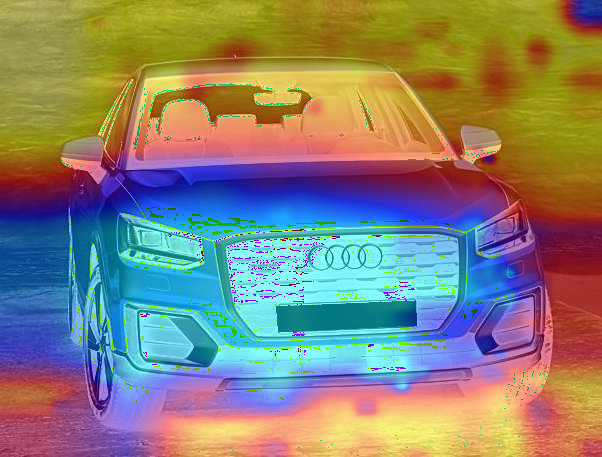
\includegraphics[width=\linewidth]{img/220_false.png}
		\caption{Ejemplo mal clasificado para el modelo DenseNet-121 refinado para
			la especificidad Marca-Modelo.}
		\label{fig:ex-densenet-refine-1}
	\end{subfigure}%
	\qquad
	\begin{subfigure}
		{.45\textwidth}
		\centering
		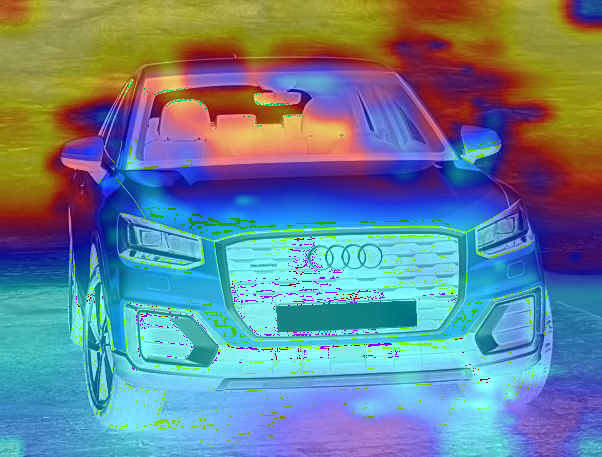
\includegraphics[width=\linewidth]{img/220_true.png}
		\caption{Ejemplo bien clasificado para el modelo DenseNet-121 refinado con
			regularización para Marca-Modelo.}
		\label{fig:ex-densenet-refine-2}
	\end{subfigure}
	\caption{Comparación de clasificación para el caso sin regularizar (a) frente
		al regularizado (b) para DenseNet-121 para la especificidad Marca-Modelo.}
	\label{fig:ex-densenet-refine}
\end{figure}

Esta vez, al tratar con una especificidad más fina, el logotipo de la marca no parece
ser suficiente criterio para detecta también el modelo, ampliando el área de
estudio (\autoref{fig:ex-densenet-refine}). Al emplear el regularizador topológico
vemos que el modelo se centra más en otros aspectos como los retrovisores o el techo
del coche frente a la versión sin regularizar.

\begin{figure}[H]
	\centering
	% First Column
	\begin{subfigure}
		{.5\textwidth}
		\centering
		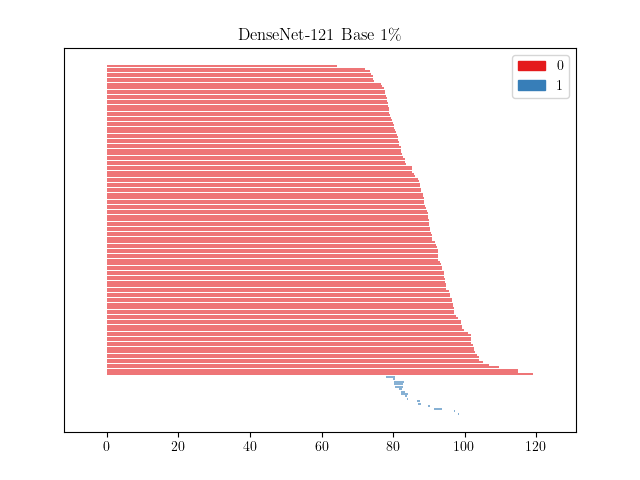
\includegraphics[width=\linewidth]{img/bar_densenet_base_0.01.png}
	\end{subfigure}%
	\begin{subfigure}
		{.5\textwidth}
		\centering
		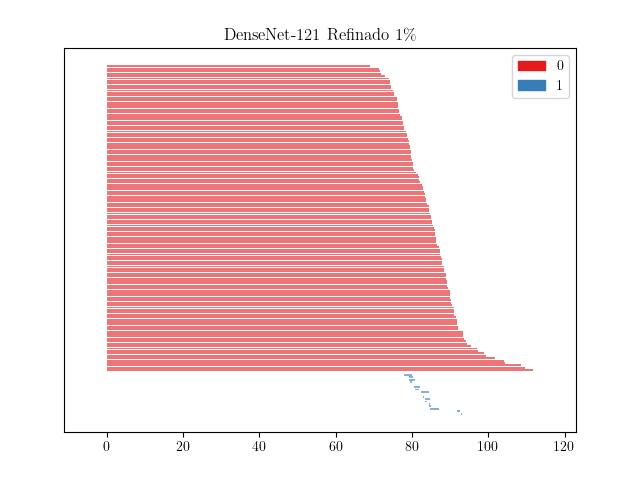
\includegraphics[width=\linewidth]{img/bar_densenet_refine_0.01.png}
	\end{subfigure}
	\begin{subfigure}
		{.5\textwidth}
		\centering
		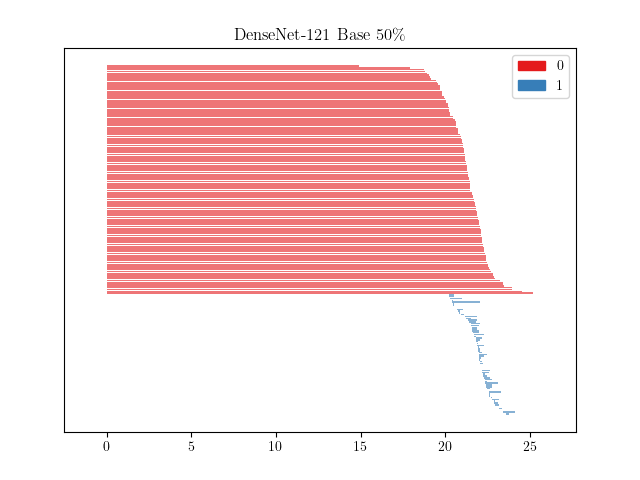
\includegraphics[width=\linewidth]{img/bar_densenet_base_0.50.png}
	\end{subfigure}%
	\begin{subfigure}
		{.5\textwidth}
		\centering
		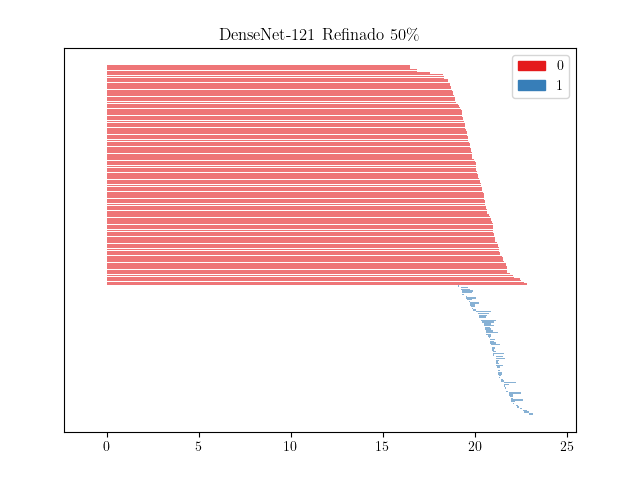
\includegraphics[width=\linewidth]{img/bar_densenet_refine_0.50.png}
	\end{subfigure}
	\begin{subfigure}
		{.5\textwidth}
		\centering
		\includegraphics[width=\linewidth]{img/bar_densenet_base_1.00.png}
	\end{subfigure}%
	\begin{subfigure}
		{.5\textwidth}
		\centering
		\includegraphics[width=\linewidth]{img/bar_densenet_refine_1.00.png}
	\end{subfigure}
	
	\caption{Comparación de los códigos de barras del modelo DenseNet-121 para el
		refinamiento en la especificidad Marca-Modelo sin regularización (izquierda)
		frente al modelo refinado con regularización (derecha). La figura muestra los códigos
		de barras para el conjunto de test tras avanzar un $1\%$ (arriba), un $50\%$ (centro)
		y el $100\%$ (abajo) de la red.}
	\label{fig:densenet-refine-bc}
\end{figure}

\subsection{Mejora en transferibilidad}

\paragraph{Transferencia EfficientNet-B0: Marca $\to$ Marca-Modelo}

La \autoref{tab:efficientnet-transfer} muestra resultados interesantes en relación
a cómo la topología afecta a la transferencia de conocimiento. Al aumentar la
granularidad del conjunto de clases y la acción del regularizador topológico
para aumentar la persistencia total normalizada de los datos, vemos que la capacidad
de clasificación del modelo mejora notablemente frente a la alternativa sin regularizar.
En el caso donde el valor $\alpha = -0.01$, el modelo llega a mejorar la exactitud
del modelo más de un 4\% y el F1-Score más de un 5\% por encima de la transferencia
base.

\begin{table}[H]
	\centering
	\begin{adjustbox}
		{width=0.8\textwidth}
		\begin{tabular}{|c|c|c|c|c|c|}
			\hline
			\textbf{Modelo}           & $\alpha$ & \textbf{Exactitud} & \textbf{Precisión} & \textbf{Sensibilidad} & \textbf{F1-Score} \\
			\hline
			EfficientNet-B0 Fine-Tune & 0.0      & 0.8333             & 0.7724             & 0.8053                & 0.7884            \\
			\hline
			EfficientNet-B0 Fine-Tune & -0.001   & 0.8407             & 0.7882             & 0.8162                & 0.8018            \\
			\hline
			EfficientNet-B0 Fine-Tune & -0.005   & 0.8407             & 0.7959             & 0.8193                & 0.8074            \\
			\hline
			EfficientNet-B0 Fine-Tune & -0.01    & \textbf{0.8741}    & \textbf{0.8276}    & \textbf{0.8522}       & \textbf{0.8397}   \\
			\hline
			EfficientNet-B0 Fine-Tune & -0.05    & 0.7963             & 0.7379             & 0.7624                & 0.7499            \\
			\hline
			EfficientNet-B0 Fine-Tune & -0.1     & 0.6000             & 0.5200             & 0.5631                & 0.5405            \\
			\hline
			EfficientNet-B0 Fine-Tune & -0.5     & 0.0222             & 0.0006             & 0.0218                & 0.0011            \\
			\hline
			EfficientNet-B0 Fine-Tune & -1.0     & 0.0148             & 0.0010             & 0.0103                & 0.0016            \\
			\hline
		\end{tabular}
	\end{adjustbox}
	\caption{Comparación de métricas tras un proceso de \textit{fine-tuning} del modelo
		EfficientNet-B0 desde la especificidad Marca hacia la especificidad Marca-Modelo
		para distintos valores de $\alpha$ en el término de regularización.}
	\label{tab:efficientnet-transfer}
\end{table}

Los resultados de las métricas se ven reforzados por las tendencias en la
\autoref{fig:efficientnet-transfer}. Aunque apenas veamos diferencias en la evolución
de la persistencia total (\autoref{fig:efficientnet-transfer-1}), la
persistencia total normalizada muestra unos valores mayores en la parte final
respecto a la transferencia base (\autoref{fig:efficientnet-transfer-2}). Este hecho
es resultado del esfuerzo en aumentar la complejidad topológica, mostrando una
relación directa entre una clasificación más fina y la topología de los datos. Una
diferencia que vemos respecto a los resultados obtenidos en la \autoref{fig:efficientnet-2}
es la ausencia de una mayor complejidad en otras etapas de la red. Al estar
considerando solamente la salida final de la red en el regularizador, el optimizador
solo parece centrarse en complicar la topología de dichas salidas. En
consecuencia, podría ser interesante plantear este concepto con activaciones de varias
capas de la red.

\begin{figure}[H]
	\centering
	\begin{subfigure}
		{.5\textwidth}
		\centering
		\includegraphics[width=\linewidth]{img/exp_transfer_efficientnet.png}
		\caption{Persistencia total normalizada según el porcentaje de avance en la
			red para el modelo EfficientNet-B0 transferido a Marca-Modelo.}
		\label{fig:efficientnet-transfer-1}
	\end{subfigure}%
	\begin{subfigure}
		{.5\textwidth}
		\centering
		\includegraphics[width=\linewidth]{img/exp_transfer_efficientnet_norm.png}
		\caption{Persistencia total normalizada según el porcentaje de avance en la
			red para el modelo EfficientNet-B0 transferido a Marca-Modelo.}
		\label{fig:efficientnet-transfer-2}
	\end{subfigure}
	\caption{Comparación de la persistencia total (a) y la persistencia total
		normalizada (b) para EfficientNet-B0 transferido con SGD y un tamaño de lote
		32 en función del porcentaje de avance de los datos a través de la red desde
		la especificidad Marca a Marca-Modelo.}
	\label{fig:efficientnet-transfer}
\end{figure}

Si observamos la \autoref{fig:ex-efficientnet-transfer}, vemos que la transferencia
hacia el mismo \textit{dataset} con una clasificación más fina, el modelo necesita
ampliar el área donde se enfoca. En particular, vemos que el modelo regularizado
logra tener un enfoque más homogéneo en la parrilla del vehículo a cambio de introducir
ciertos artefactos lineales.

\begin{figure}[H]
	\centering
	\begin{subfigure}
		{.45\textwidth}
		\centering
		\includegraphics[width=\linewidth]{img/154_false.png}
		\caption{Ejemplo mal clasificado para el modelo EfficientNet-B0 transferido
			desde la especificidad Marca a Marca-Modelo.}
		\label{fig:ex-efficientnet-transfer-1}
	\end{subfigure}%
	\qquad
	\begin{subfigure}
		{.45\textwidth}
		\centering
		\includegraphics[width=\linewidth]{img/154_true.png}
		\caption{Ejemplo bien clasificado para el modelo EfficientNet-B0 transferido
			desde la especificidad Marca a Marca-Modelo.}
		\label{fig:ex-efficientnet-transfer-2}
	\end{subfigure}
	\caption{Comparación de clasificación para el caso sin regularizar (a) frente
		al regularizado (b) para la transferencia de EfficientNet-B0 a Marca-Modelo.}
	\label{fig:ex-efficientnet-transfer}
\end{figure}

Como consecuencia directa de aumentar la complejidad topológica de los datos, los
códigos de barras en el final de la red regularizada muestra intervalos algo más
numerosos y de longitud similar, de forma que disponemos de una mayor
persistencia total normalizada (\autoref{fig:efficientnet-transfer-bc}).

\begin{figure}[H]
	\centering
	% First Column
	\begin{subfigure}
		{.5\textwidth}
		\centering
		\includegraphics[width=\linewidth]{img/bar_efficientnet_trans_base_0.01.png}
	\end{subfigure}%
	\begin{subfigure}
		{.5\textwidth}
		\centering
		\includegraphics[width=\linewidth]{img/bar_efficientnet_trans_reg_0.01.png}
	\end{subfigure}
	\begin{subfigure}
		{.5\textwidth}
		\centering
		\includegraphics[width=\linewidth]{img/bar_efficientnet_trans_base_0.50.png}
	\end{subfigure}%
	\begin{subfigure}
		{.5\textwidth}
		\centering
		\includegraphics[width=\linewidth]{img/bar_efficientnet_trans_reg_0.50.png}
	\end{subfigure}
	\begin{subfigure}
		{.5\textwidth}
		\centering
		\includegraphics[width=\linewidth]{img/bar_efficientnet_trans_base_1.00.png}
	\end{subfigure}%
	\begin{subfigure}
		{.5\textwidth}
		\centering
		\includegraphics[width=\linewidth]{img/bar_efficientnet_trans_reg_1.00.png}
	\end{subfigure}
	
	\caption{Comparación de los códigos de barras del modelo EfficientNet-B0 para
		la transferencia de la especificidad Marca a Marca-Modelo sin regularización (izquierda)
		frente al modelo transferido con regularización (derecha). La figura muestra los
		códigos de barras para el conjunto de test tras avanzar un $1\%$ (arriba), un
		$50\%$ (centro) y el $100\%$ (abajo) de la red.}
	\label{fig:efficientnet-transfer-bc}
\end{figure}

\paragraph{Transferencia Densenet-121: Marca-Modelo $\to$ Marca}

Por su parte, la transferencia desde Marca-Modelo a Marca ha mostrado métricas
más mucho más altas que las vistas en la transferencia opuesta (\autoref{tab:densenet-transfer}).
A pesar de la similitud entre los resultados obtenidos, vemos que los mejores
resultados los han obtenido las variantes para los valores de $\alpha$ iguales a
0.001 y 0.005. Más aún, es interesante ver cómo alteraciones similares de la
topología de los datos pueden llevar los resultados obtenidos a los mismos
valores. %Una hipótesis podría sugerir que la alteración de la homología persistente en CNNs converge de manera discreta a las mismas estructuras en función de varios umbrales de $\alpha$.

\begin{table}[H]
	\centering
	\begin{adjustbox}
		{width=0.8\textwidth}
		\begin{tabular}{|c|c|c|c|c|c|}
			\hline
			\textbf{Modelo}        & $\alpha$ & \textbf{Exactitud} & \textbf{Precisión} & \textbf{Sensibilidad} & \textbf{F1-Score} \\
			\hline
			DenseNet-121 Fine-Tune & 0.0      & 0.9907             & 0.9816             & 0.9864                & 0.9840            \\
			\hline
			DenseNet-121 Fine-Tune & 0.001    & \textbf{0.9938}    & \textbf{0.9834}    & \textbf{0.9882}       & \textbf{0.9857}   \\
			\hline
			DenseNet-121 Fine-Tune & 0.005    & \textbf{0.9938}    & \textbf{0.9834}    & \textbf{0.9882}       & \textbf{0.9857}   \\
			\hline
			DenseNet-121 Fine-Tune & 0.01     & 0.9876             & 0.9747             & 0.9812                & 0.9779            \\
			\hline
			DenseNet-121 Fine-Tune & 0.05     & 0.9443             & 0.8895             & 0.9077                & 0.8983            \\
			\hline
			DenseNet-121 Fine-Tune & 0.1      & 0.8111             & 0.6628             & 0.7252                & 0.6919            \\
			\hline
			DenseNet-121 Fine-Tune & 0.5      & 0.0194             & 0.0738             & 0.0738                & 0.0287            \\
			\hline
			DenseNet-121 Fine-Tune & 1.0      & 0.0743             & 0.0048             & 0.0546                & 0.0086            \\
			\hline
		\end{tabular}
	\end{adjustbox}
	\caption{Comparación de métricas tras un proceso de \textit{fine-tuning} del modelo
		DenseNet-121 desde la especificidad Marca-Modelo hacia la especificidad Marca para
		distintos valores de $\alpha$ en el término de regularización.}
	\label{tab:densenet-transfer}
\end{table}

Pese a la poca diferencia entre métricas, los cambios en homología persistente muestran
varios aspectos de interés. En esta ocasión, la simplificación de la persistencia
total normalizada se ha reflejado en la persistencia total a través de una simplificación
al comienzo de la red, tal y como muestra la \autoref{fig:densenet-transfer-1}. Por
otra parte, la \autoref{fig:densenet-transfer-2} muestra claramente como el
regularizador ha funcionado como se esperaba. Es curioso ver cómo para los casos
donde $\alpha = 0.001$ y $\alpha = 0.005$, cuyas métricas son idénticas, obtenemos
diferencias en complejidad topológica tan notables.

\begin{figure}[H]
	\centering
	\begin{subfigure}
		{.5\textwidth}
		\centering
		\includegraphics[width=\linewidth]{img/exp_transfer_densenet.png}
		\caption{Persistencia total según el porcentaje de avance en la red para el
			modelo DenseNet-121 transferido desde la especificidad Marca-Modelo a Marca.}
		\label{fig:densenet-transfer-1}
	\end{subfigure}%
	\begin{subfigure}
		{.5\textwidth}
		\centering
		\includegraphics[width=\linewidth]{img/exp_transfer_densenet_norm.png}
		\caption{Persistencia total normalizada según el porcentaje de avance en la
			red para el modelo DenseNet-121 transferido desde la especificidad Marca-Modelo
			a Marca.}
		\label{fig:densenet-transfer-2}
	\end{subfigure}
	\caption{Comparación de la persistencia total (a) y la persistencia total
		normalizada (b) para DenseNet-121 transferido con SGD y un tamaño de lote 32
		en función del porcentaje de avance de los datos a través de la red desde la
		especificidad Marca-Modelo a Marca.}
	\label{fig:densenet-transfer}
\end{figure}

Finalmente, los códigos de barras en la \autoref{fig:densenet-transfer-bc} reflejan
el comportamiento esperado en las capas finales, donde el modelo regularizado
muestra intervalos de persistencia más cortos que su par (\autoref{fig:densenet-transfer-bc}).
Pese al aumento de persistencia total en las capas iniciales, los códigos de
barras no parecen dar una respuesta a esta cuestión.

\begin{figure}[H]
	\centering
	% First Column
	\begin{subfigure}
		{.5\textwidth}
		\centering
		\includegraphics[width=\linewidth]{img/bar_densenet_trans_base_0.01.png}
	\end{subfigure}%
	\begin{subfigure}
		{.5\textwidth}
		\centering
		\includegraphics[width=\linewidth]{img/bar_densenet_trans_reg_0.01.png}
	\end{subfigure}
	\begin{subfigure}
		{.5\textwidth}
		\centering
		\includegraphics[width=\linewidth]{img/bar_densenet_trans_base_0.50.png}
	\end{subfigure}%
	\begin{subfigure}
		{.5\textwidth}
		\centering
		\includegraphics[width=\linewidth]{img/bar_densenet_trans_reg_0.50.png}
	\end{subfigure}
	\begin{subfigure}
		{.5\textwidth}
		\centering
		\includegraphics[width=\linewidth]{img/bar_densenet_trans_base_1.00.png}
	\end{subfigure}%
	\begin{subfigure}
		{.5\textwidth}
		\centering
		\includegraphics[width=\linewidth]{img/bar_densenet_trans_reg_1.00.png}
	\end{subfigure}
	
	\caption{Comparación de los códigos de barras del modelo DenseNet-121 para la
		transferencia de la especificidad Marca-Modelo a Marca sin regularización (izquierda)
		frente al modelo con regularización (derecha). La figura muestra los códigos de
		barras para el conjunto de test tras avanzar un $1\%$ (arriba), un $50\%$ (centro)
		y el $100\%$ (derecha) de la red.}
	\label{fig:densenet-transfer-bc}
\end{figure}

A diferencia de la transferencia anterior, al reducir el número de clases vemos
que el modelo focaliza su análisis en un área más concentrada (\autoref{fig:ex-densenet-transfer}).
La \autoref{fig:ex-densenet-transfer-2} muestra un área de enfoque más reducida que
el caso sin regularizar, centrándose en las características más relevantes y
evitando otras que podrían introducir ruido.

\begin{figure}[H]
	\centering
	\begin{subfigure}
		{.45\textwidth}
		\centering
		\includegraphics[width=\linewidth]{img/94_false.png}
		\caption{Ejemplo mal clasificado para el modelo DenseNet-121 transferido
			desde la especificidad Marca-Modelo a Marca.}
		\label{fig:ex-densenet-transfer-1}
	\end{subfigure}%
	\qquad
	\begin{subfigure}
		{.45\textwidth}
		\centering
		\includegraphics[width=\linewidth]{img/94_true.png}
		\caption{Ejemplo bien clasificado para el modelo DenseNet-121 transferido
			desde la especificidad Marca-Modelo a Marca.}
		\label{fig:ex-densenet-transfer-2}
	\end{subfigure}
	\caption{Comparación de clasificación para el caso sin regularizar (a) frente
		al regularizado (b) para la transferencia de DenseNet-121 a Marca.}
	\label{fig:ex-densenet-transfer}
\end{figure}

\subsection{Impacto de la regularización topológica en CNNs}

La implementación de un regularizador topológico en modelos como EfficientNet-B0
y DenseNet-121 ha demostrado ser prometedora, mejorando tanto la clasificación como
la transferencia de conocimiento. Este enfoque ajusta la complejidad topológica
de los datos, lo que parece reflejarse en la mejora general del rendimiento del modelo.

Para el modelo EfficientNet-B0, el uso del regularizador topológico ha mostrado
una mejora leve pero significativa en comparación con versiones sin
regularización. Las observaciones realizadas indican que ajustar la topología,
principalmente en etapas finales del aprendizaje, puede afinar la capacidad del modelo
para diferenciar entre clases y por tanto haciendo más efectiva la clasificación
final. Esto se ve en cómo el modelo regularizado presenta intervalos más cortos
de persistencia en instantes más cercanos al final del proceso de inferencia.

En el caso de DenseNet-121, la aplicación del regularizador ha tenido un impacto
considerable, optimizando de manera efectiva la estructura de los datos para
mejorar el rendimiento del modelo. Los cambios sutiles en la homología al final de
la red han demostrado ser importantes, reduciendo la cantidad de componentes
conexas y aumentando la duración de las clases de homología persistente de
dimensiones superiores, lo que sugiere una manipulación estratégica de la topología
para beneficiar la tarea de clasificación.

En términos de transferibilidad, los estudios sobre EfficientNet-B0 y DenseNet-121
muestran que el regularizador topológico no solo mejora la clasificación en el
dominio original, sino que también facilita la transferencia de conocimiento al menos
hacia dominios de diferente granularidad. Esto se muestra en la mejora de la
clasificación cuando se aumenta la granularidad de las clases, y cómo la complejidad
topológica ajustada al final del proceso contribuye de manera notable a estos resultados.
La relación entre una clasificación más precisa y la topología de los datos
sugiere que enfocarse en optimizar la topología en las salidas finales puede ser
una estrategia eficaz.

Sin embargo, la selección del valor de $\alpha$ para el regularizador ha mostrado
ser relevante y debe hacerse con cuidado. Un valor inadecuado puede llevar a
resultados subóptimos, indicando la sensibilidad de la técnica y la necesidad de
entender profundamente cómo las modificaciones topológicas influencian el aprendizaje.
Por este motivo, el estudio realizado sugiere escoger valores de $\alpha$ entre $0
.001$ y $0.1$.

\endinput
%--------------------------------------------------------------------
% FIN DEL CAPÍTULO.
%--------------------------------------------------------------------